\documentclass{jsarticle}
\usepackage[dvipdfmx]{graphicx}
\usepackage{amsmath,amssymb}
\usepackage{amsthm}
\newtheorem{df}{[定義]}[section]
\newtheorem{thm}{定理}[section]
\newtheorem{lem}{補題}[section]
\newtheorem{ex}{例}[section]
\title{リーマンゼータ関数 ノート1}

\author{}
\date{}
\begin{document}
\maketitle
\noindent
1.ゼータ関数の収束域\\
2.オイラーの定数\\
3.ゼータ関数のオイラーの積表示\\
4.素数の逆数和\\
5.\(s>0\)への解析接続\\
6.積分表示\\
7.関数等式\\
8.特殊値\\
9.アダマール積\\
10.素数分布\\
11.数論的関数との関係\\
12.明示公式\\
13.素数定理\\
\\
\\
\\
\\
\\
〇参考文献\\
・「素数とゼータ関数」 小山 信也 /共立出版\\
・「ゼータへの招待」 黒川 信重 小山 信也 /日本評論社\\
・「オイラーとリーマンのゼータ関数」 黒川 信重 /日本評論社\\
・「解析的整数論1」 カール・ジーゲル /岩波書店\\
・「複素解析」 エリアス・M.スタイン ラミ・シャカルチ /日本評論社\\
・「複素解析」 L.V.アールフォルス /現代数学社\\
・「リーマンゼータ関数と保型波動」 本橋 洋一 /共立出版\\
・「リーマンのゼータ関数」 松本耕二 /朝倉書店
\newpage
\section{ゼータ関数の収束域}
ゼータ関数はディリクレ級数表示で以下のように定義される。
\begin{equation}
\zeta(s):=\sum_{n=1}^{\infty}\frac{1}{n^{s}}
\end{equation}
このディリクレ級数表示のゼータ関数の収束について以下の定理が成り立つ。\\

<定理1.1>\\
(1)級数(1.1)は\(s>1\)において収束し、\(s\leq1\)において発散する。\\
(2)\(s=1\)のときの時の級数(1.1)の部分和の挙動は以下のとおりである。
\begin{equation}
\sum_{n<x}\frac{1}{n}\sim\log x\hspace{5mm}(x\rightarrow\infty)
\end{equation}
〇証明\\
はじめに\(s>1\)で収束することを示す。正の実数\(t\)に対し、\(t\leq n\)なる整数を\(n\)とおく。このとき、\(n-1<t\leq n\)となり、\(s\geq0\)ならば、\(n^{-s}\leq t^{-s}<(n-1)^{-s}\)が成り立つ。よって
\[\zeta(s)=\sum_{n=1}^{\infty}\frac{1}{n^{s}}=1+\sum_{n=2}^{\infty}\frac{1}{n^{s}}\]
となるが、ここでグラフを描くと明らかであるが、\(\displaystyle\sum_{n=2}^{\infty}\frac{1}{n^{s}}\leq\int_{1}^{\infty}\frac{1}{t^{s}}dt\)であるから\(s>1\)のとき
\[\zeta(s)\leq1+\int_{1}^{\infty}\frac{1}{t^{s}}dt=1+\left[\frac{t^{1-s}}{1-s}\right]_{1}^{\infty}=1+\frac{1}{s-1}=\frac{s}{s-1}\]
ゆえに級数(1.1)は\(s>1\)のとき、収束する。また、\(s>1\)のとき、発散することは(2)を示せば十分である。以下(2)を示す。(1)と同様にして上限は
\[\displaystyle\sum_{n<x}\frac{1}{n}=1+\sum_{2\leq n<x}\leq1+\int_{1}^{x}\frac{1}{t}dt=1+\left[\log t\right]_{1}^{x}=1+\log x\]
一方、正の実数tに対し、nはt以上の最小の整数であったから、\(n\leq t+1\)より、\\
\(\frac{1}{t+1}\leq\frac{1}{n}\)が成り立つから
\[\int_{n-1}^{n}\frac{1}{t+1}\leq\frac{1}{n}\]
両辺を足し合わせて
\[\displaystyle\sum_{n<x}\frac{1}{n}\geq\sum_{n<x}\int_{n-1}^{n}\frac{1}{t+1}dt=\int_{0}^{x-1}\frac{1}{t+1}dt=\Bigl[\log(t+1)\Bigr]_{0}^{x-1}=\log x\]
以上より、
\[\log x\leq\sum_{n<x}\frac{1}{n}\leq1+\log x\]
であるから、はさみうちの原理により、
\[\displaystyle\lim_{x\rightarrow\infty}\frac{\sum_{n<x}\frac{1}{n}}{\log x}=1\]
が成り立つ。\\
この\(\zeta(1)\)ののときの発散することの証明として有名なオレームの証明があり、その証明方法は
\[\zeta(1)=1+\frac{1}{2}+\left(\frac{1}{3}+\frac{1}{4}\right)+\left(\frac{1}{5}+\frac{1}{6}+\frac{1}{7}+\frac{1}{8}\right)+\cdots\]
\[\hspace{15mm}>1+\frac{1}{2}+\left(\frac{1}{4}+\frac{1}{4}\right)+\left(\frac{1}{8}+\frac{1}{8}+\frac{1}{8}+\frac{1}{8}+\frac{1}{8}\right)+\cdots\]
\[=1+\frac{1}{2}+\frac{1}{2}+\frac{1}{2}+\frac{1}{2}+\cdots=\infty\]
と簡潔に証明される。また、sの値により収束・発散することはマクローリン・コーシーの判定法からもただちに分かる。
\[\sum_{n=1}^{\infty}\frac{1}{n^{s}}\longleftrightarrow\int_{1}^{\infty}\frac{1}{t^{s}}dt=\frac{1}{1-x}t^{1-x}\Big|_{1}^{\infty}\hspace{10mm}(s\neq1)\]







\setcounter{equation}{0}
\section{オイラーの定数}
オイラーがみつけたオイラー定数について定義し、ゼータ関数との関係性を見ていく。\\
<定理2.1>\\
次式を満たす定数\(\gamma\)が存在する。
\begin{equation}
\sum_{k=1}^{n}\frac{1}{k}-\log n=\gamma+O\left(\frac{1}{n}\right)\hspace{10mm}(n\rightarrow\infty)
\end{equation}
〇証明\\
\(y=\frac{1}{x}\)のグラフと階段グラフ\(y=\frac{1}{\lfloor x\rfloor}\)を比較することにより、
\[\log n<\sum_{k=1}^{n-1}\frac{1}{k}\]
が分かる。この両者の差は、図1のグラフのオレンジ色の部分に相当する面積である。この領域を
\[S_{n}=\sum_{k=1}^{n-1}\frac{1}{k}-\log n\]
と置く。この図形を左側に移動させ、\(0<x<1\)の領域で考えることにより、\(S_{n}<1\)であることが分かる。また、この\(S_{n}\)はnに対して単調増加かつ上に有界であるから、\(n\rightarrow\infty\)において収束する。その収束値を\(\gamma\)とおく。
\[\gamma-S_{n}\]は\(\gamma\)の表す面積(無限集合)から、有限部分でのn個分の面積を引いたものである。元のグラフを左に平行移動させた図2のグラフをみればわかる通り、これは\(\frac{1}{n}\)未満に収まる。したがって
\[0<\gamma-S_{n}<\frac{1}{n}\]
が成り立つので、定理が示された。

\begin{figure}[h]
  \begin{minipage}{0.5\hsize}
    \begin{center}
      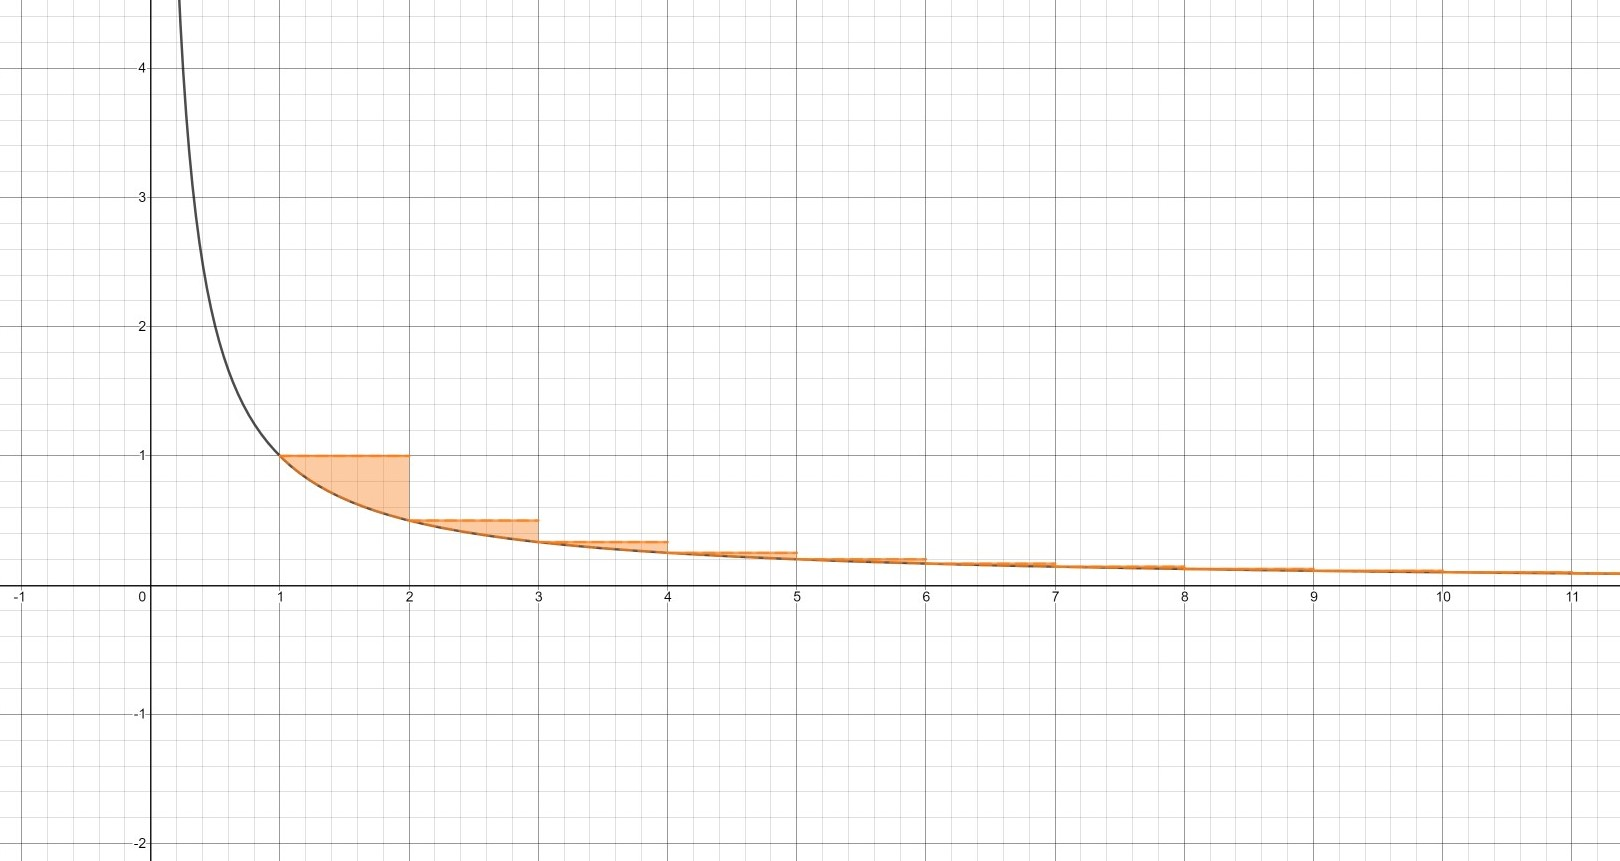
\includegraphics[width=60mm]{zeta-photo1.jpg}
     
    \end{center}
    \caption{}
   
  \end{minipage}
  \begin{minipage}{0.5\hsize}
    \begin{center}
      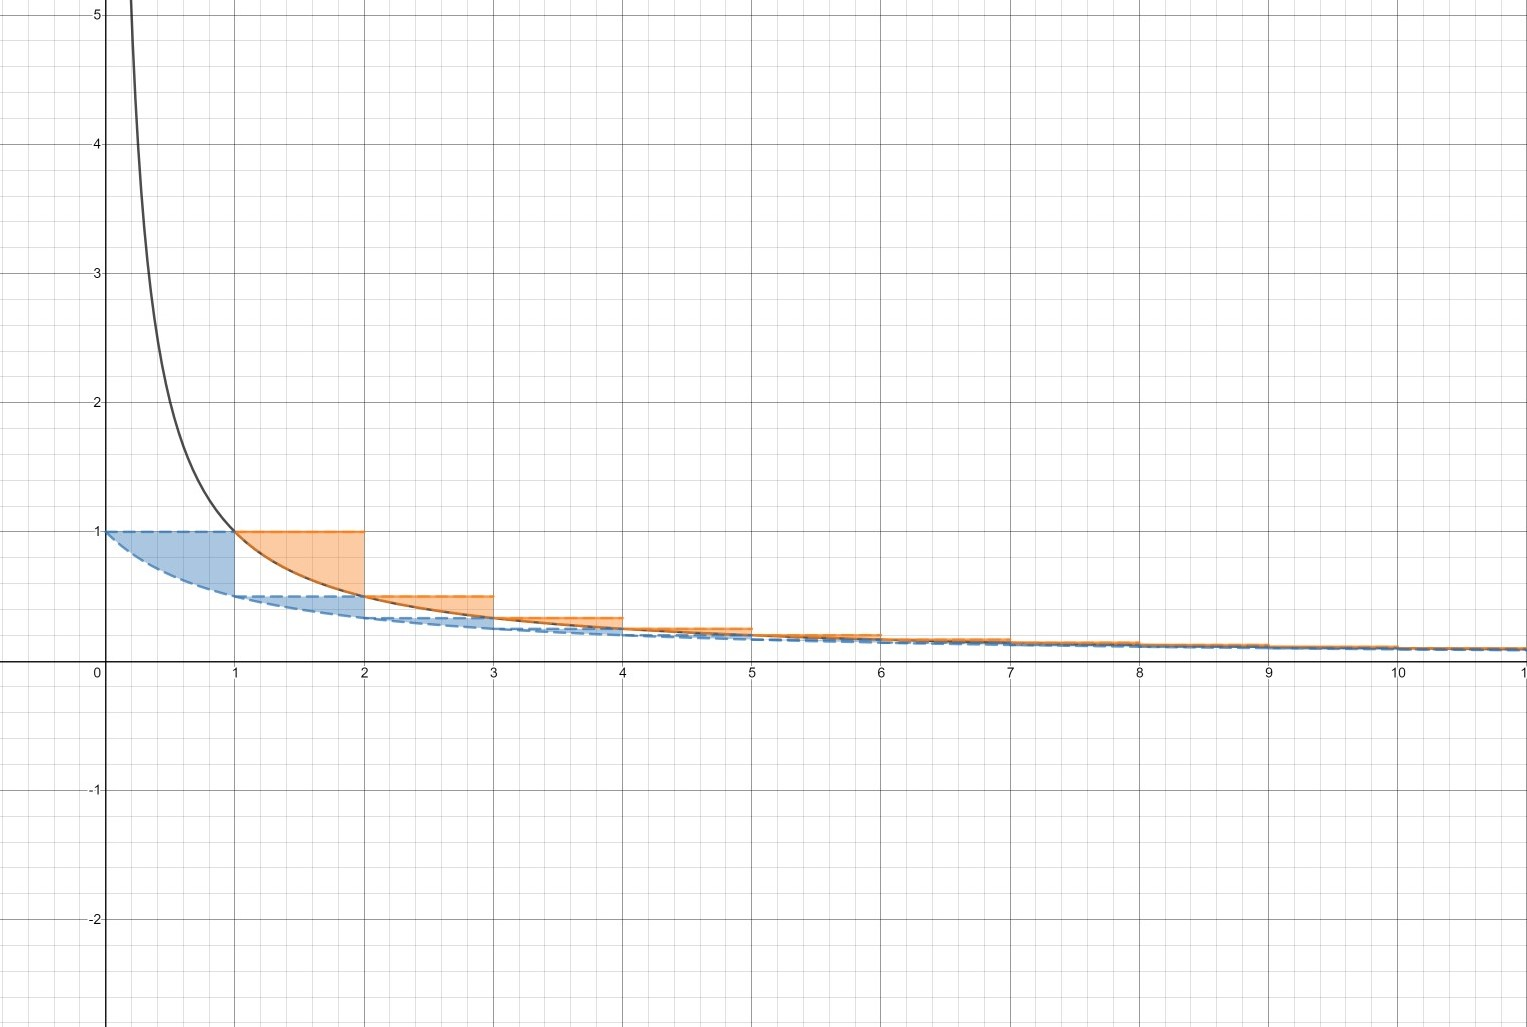
\includegraphics[width=60mm]{zeta-photo2.jpg}
    \end{center}
    \caption{}
  \end{minipage}
\end{figure}
次にゼータ関数を含めた表示を見ていく。\\
\\
<定理2.2>\\
\begin{equation}
\gamma=\sum_{n=2}^{\infty}\frac{(-1)^{n}}{n}\zeta(n)
\end{equation}
が成り立つ。\\
〇証明\\
対数関数をマクローリン展開して得られる式
\[\ln\frac{x+1}{x}=\sum_{n=1}^{\infty}\frac{(-1)^{n-1}}{n}\cdot\frac{1}{m^{n}}\]
について\(m=1,2,\cdots,M\)まで足し合わせると
\[\ln\prod_{n=1}^{M}\frac{m+1}{m}=\ln(M+1)=\sum_{n=1}^{\infty}\frac{(-1)^{n-1}}{n}\left(\sum_{m=1}^{M}\frac{1}{m^{n}}\right)\]
\[\hspace{21mm}=1+\frac{1}{2}+\cdots+\frac{1}{M}+\sum_{n=2}^{\infty}\frac{(-1)^{n-1}}{n}\cdot\sum_{m=1}^{\infty}\frac{1}{m^{n}}\]
となる。移項することにより
\[1+\frac{1}{2}+\cdots+\frac{1}{M}-\ln(M+1)=\sum_{n=2}^{\infty}\frac{(-1)^{n}}{n}\cdot\sum_{n=1}^{\infty}\frac{1}{m^{n}}\]
両辺から\(\ln(M+1)-\ln M\)を加えて
\[1+\frac{1}{2}+\cdots+\frac{1}{M}-\ln M=\sum_{n=2}^{\infty}\frac{(-1)^{n}}{n}\cdot\sum_{m=1}^{\infty}\frac{1}{m^{n}}+\ln\left(1+\frac{1}{M}\right)\]
を得る。よって\(M\rightarrow\infty\)とすると
\[\gamma=\sum_{n=2}^{\infty}\frac{(-1)^{n}}{n}\zeta(n)\]
\\
<定理2.3>\\
ゼータ関数についての極限公式
\begin{equation}
\gamma=\lim_{s\rightarrow1}\left(\zeta(s)-\frac{1}{s-1}\right)
\end{equation}
が成り立つ。\\
〇証明
\(s>1\)に対し
\begin{eqnarray*}
\int_{1}^{M+1}\left(\frac{1}{\lfloor x\rfloor^{s}}-\frac{1}{x^{s}}\right)dx &=&  \sum_{m=1}^{M}\frac{1}{m^{s}}-\left[\frac{x^{1-s}}{1-s}\right]_{1}^{M+1}\\
&=& \sum_{m=1}^{M}\frac{1}{m^{s}}-\frac{1-(M+1)^{1-s}}{s-1}
\end{eqnarray*}
となるので\(M\rightarrow\infty\)として
\[\int_{1}^{M+1}\left(\frac{1}{\lfloor x\rfloor^{s}}-\frac{1}{x^{s}}\right)dx=\zeta(s)-\frac{1}{s-1}\]
を得る。したがって
\begin{eqnarray*}
\lim_{s\rightarrow1}\left(\zeta(s)-\frac{1}{s-1}\right) &=&\int_{1}^{\infty}\left(\frac{1}{\lfloor x\rfloor}-\frac{1}{x}\right)dx\\
&=&\lim_{M\rightarrow\infty}\int_{1}^{M+1}\left(\frac{1}{\lfloor x\rfloor}-\frac{1}{x}\right)dx\\
&=&\lim_{M\rightarrow\infty}\left(1+\cdots+\frac{1}{M}-\ln(M+1)\right)\\
&=&\gamma
\end{eqnarray*}
となる。





\setcounter{equation}{0}
\section{ゼータ関数のオイラー積表示}
\(a(n)\)を乗法的関数である数論的関数とするとこれを母関数とするディリクレ級数は
\begin{equation}
\sum_{n=1}^{\infty}\frac{a(n)}{n^{s}}=\prod_{p;\mathrm{prime}}\left(1+\frac{a(p)}{p^{s}}+\frac{a(p^{2})}{p^{2s}}+\cdots\right)
\end{equation}
が成り立つことが知られている。特に\(a(n)\)が完全乗法的関数のとき
\begin{equation}
\sum_{n=1}^{\infty}\frac{a(n)}{n^{s}}=\prod_{p;\mathrm{prime}}\left(1+\frac{a(p)}{p^{s}}+\frac{a(p^{2})}{p^{2s}}+\cdots\right)
=\prod_{p;\mathrm{prime}}\frac{1}{1-\frac{a(p)}{p^{s}}}
\end{equation}
と表される。ここで特に\(a(n)=1\)のとき左辺はゼータ関数となる。\\
<定理3.1>\\
\begin{equation}
\sum_{n=1}^{\infty}\frac{1}{n^{s}}=\prod_{p;\mathrm{prime}}\frac{1}{1-p^{-s}}
\end{equation}
が成り立つ。\\
〇証明1\\
\begin{eqnarray*}
\prod_{p}\frac{1}{1-p^{-s}}&=&\prod_{i=1}\sum_{k_{i}=0}^{\infty}\left(\frac{1}{p_{i}^{s}}\right)^{k_{i}}=\prod_{p}\sum_{k_{i}=0}^{\infty}\frac{1}{p_{i}^{sk_{i}}}\\
&=&\sum_{k_{1}=0}^{\infty}\frac{1}{p_{1}^{sk_{1}}}\cdot\sum_{k_{2}=0}^{\infty}\frac{1}{p_{2}^{sk_{2}}}\cdot\cdots\cdot\sum_{k_{N}=0}^{\infty}\frac{1}{p_{N}^{sk_{N}}}\cdot\cdots\\
&=&\sum_{k_{1}=0}^{\infty}\sum_{k_{2}=0}^{\infty}\sum_{k_{3}=0}^{\infty}\cdots\left(\frac{1}{p_{1}^{k_{1}}}\frac{1}{p_{2}^{k_{2}}}\cdots\frac{1}{p_{N}^{k_{N}}}\cdots\right)^{s}
\end{eqnarray*}
左辺は素因数のすべての組み合わせについて和をとっていることが分かる。素因数分解の一意性より左辺は\(\sum\frac{1}{n^{s}}\)である。\\
〇証明2\\
2つ目の証明をする。こちらの方が簡単で項の入れ替えもなく理解しやすいと思う。\\
ゼータ関数のディリクレ級数表示に\(\frac{1}{2^{s}}\)を掛けてあげると
\[\frac{1}{2^{s}}\zeta(s)=\sum_{n=1}^{\infty}\frac{1}{(2n)^{s}}\]となるから、元のゼータ関数からこれを引くと
\[\zeta(s)-\frac{1}{2^{s}}\zeta(s)=\left(1-\frac{1}{2^{s}}\right)\zeta(s)=\sum_{n=1}^{\infty}\frac{1}{n^{s}}-\sum_{n=1}^{\infty}\frac{1}{(2n)^{s}}=\sum_{\substack {n=1 \\ n\neq 2k}}\frac{1}{n^{s}}\]
となる。さらにこれに\(\frac{1}{3^{s}}\)を掛けると
\[
\zeta(s)\left(1-\frac{1}{2^{s}}\right)\frac{1}{3^{s}}=\sum_{\substack{n=1\\n\neq 2k}}\frac{1}{(3n)^{s}}
\]
となるから同様にして
\[\zeta(s)\left(1-\frac{1}{2^{s}}\right)\left(1-\frac{1}{3^{s}}\right)=\sum_{\substack{n=1\\n\neq2k\\n\neq3k}}\frac{1}{n^{s}}\]
これを繰り返し用いることで
\[\zeta(s)\left(1-\frac{1}{2^{s}}\right)\left(1-\frac{1}{3^{s}}\right)\left(1-\frac{1}{5^{k}}\right)\cdots=\sum_{\substack{n=1\\n\neq2k\\n\neq3k\\ \cdots}}\frac{1}{n^{s}}=1\]
移項して
\[\zeta(s)=\frac{1}{\left(1-\frac{1}{2^{s}}\right)\left(1-\frac{1}{3^{s}}\right)\left(1-\frac{1}{5^{k}}\right)\cdots}=\prod_{p}\frac{1}{1-p^{-s}}\]





\setcounter{equation}{0}
\section{素数の逆数和}
素数が自然数のうち、どれくらい存在するのか考えるため逆数和を考えてみる。結論から言うと素数の逆数和は発散する。それに反してべき級数や平方数の無限級数は収束する。これは素数が自然数全体を占める割合は、べき級数や平方数に比べると、大きいことを意味する。\\
<定理4.1>\\
\
\begin{equation}
\sum_{p}\frac{1}{p}=\frac{1}{2}+\frac{1}{3}+\frac{1}{5}+\frac{1}{7}+\frac{1}{11}+\frac{1}{13}+\cdots=\infty
\end{equation}
〇証明
\[\sum_{n=1}^{\infty}\frac{1}{n^{s}}=\prod_{p:素数}\frac{1}{1-p^{-s}}\]
から始める。まず、両辺を対数をとり\(s>1\)で
\[\log\zeta\left(s\right)=\log\prod_{p:素数}\left(1-p^{-s}\right)^{-1}=-\sum_{p:素数}\log\left(1-p^{-s}\right)\]
ここで\(\log\left(1-x\right)\)のマクローリン展開を求めると
\(\displaystyle\log\left(1-x\right)=f(0)+f'(0)\frac{x}{1!}+f^{(2)}(0)\frac{x^{2}}{2!}+\cdots\)より
\[\log(1-x)=0-\left[\frac{1}{1-x}\right]_{x=0}\frac{x}{1!}-\left[\frac{1}{(1-x)^{2}}\right]_{x=0}\frac{x^{2}}{2!}-\left[\frac{2}{(1-x)^{3}}\right]_{x=0}\frac{x^{3}}{3!}-\cdots-\left[\frac{(m-1)!}{(1-x)^{m}}\right]_{x=0}\frac{x^{m}}{m!}\]
\[=0-x-\frac{x^{2}}{2}-\frac{x^{3}}{3}-\cdots=-\sum_{m=1}^{\infty}\frac{x^{m}}{m}\]
となる。なお、正項級数を扱っているので項の入れ替えは問題ない。またこのとき収束条件は\(|x|<1\)である。\(x=p^{-s}\)はこれを満たし、代入すると
\[\log(1-p^{-s})=-\sum_{m=1}^{\infty}\frac{p^{-ms}}{m}\]
ゆえに
\[\log\zeta(s)=-\sum_{p:素数}\log(1-p^{-s})=\sum_{p:素数}\sum_{m=1}^{\infty}\frac{1}{mp^{ms}}=\sum_{p}\left(\frac{1}{p^{s}}+\sum_{m=2}^{
\infty}\frac{1}{mp^{ms}}\right)\]
\begin{eqnarray}
=\sum_{p}\frac{1}{p^{s}}+\sum_{p}\sum_{m=2}^{\infty}\frac{1}{mp^{ms}}
\end{eqnarray}
\\
左辺は\(s\rightarrow1\)で発散するので、右辺の第二項が収束することを示せば、第1項が発散することが示される。
\[\sum_{m=2}^{\infty}\frac{1}{mp^{ms}}<\sum_{m=2}^{\infty}\frac{1}{2p^{ms}}=\frac{1}{2}\sum_{m=2}^{\infty}\frac{1}{p^{ms}}=\frac{1}{2}\frac{1}{p^{2s}}\sum_{m=0}^{\infty}\frac{1}{p^{ms}}\]
\[\left( 無限等比級数の収束値より\sum_{m=0}^{\infty}\left(p^{-s}\right)^{m}=\frac{1}{1-p^{-s}}であるから\right)=\frac{1}{2p^{2s}}\frac{1}{1-\frac{1}{p^{s}}}\]
ここで\(\frac{1}{p^{2s}}<\frac{1}{2}\)より\hspace{10mm}\(\displaystyle\frac{1}{2p^{2s}}\frac{1}{1-p^{-s}}<\frac{1}{2p^{2s}}\frac{1}{1-\frac{1}{2}}=\frac{1}{p^{2s}}\)\\
\\
よって素数全体で足し合わせると
\[\sum_{p}\sum_{m=2}^{\infty}\frac{1}{mp^{ms}}<\sum_{p}\frac{1}{p^{2s}}<\sum_{n=1}^{\infty}\frac{1}{n^{2s}}<\sum_{n=1}^{\infty}\frac{1}{n^{2}}=\frac{\pi^{2}}{6}\]
したがって\(m\leq2\)に関する和は収束することが示された。\\
これより(2)式をもとに\(s\to1\)を考えると右辺の第二項は以上より収束するが、左辺は\(\displaystyle\lim_{s\to1}\zeta(s)=\infty\)となり発散することから右辺の第一項が発散することが示された。\\
この結果からも素数が無限個あることが分かる。\\
次に実際に素数の逆数和の増大度について見ていく。\\
<定理4.2>\\
\begin{equation}
\sum_{\substack{p\leq x\\p:素数}}\frac{1}{p}\sim\log\log x\hspace{10mm}(x\to\infty)
\end{equation}
が成り立つ。\\
\\
証明する前に道具としていくつかの補題を用意する。\\
<補題4.3>\\
自然数\(m\)の素因数分解に素数\(p\)が現れる回数を\(\nu_{p}(m)\)と置く。そのとき、階乗について
\begin{equation}
\nu(n!)=\sum_{k=1}^{\infty}\left[\frac{n}{p^{k}}\right]
\end{equation}
以下ことわりがない限り\(p\)を素数とする。\\
〇証明\\
指数法則(\(z^{a+b}=z^{a}z^{b}\))より
\[\nu_{p}(n!)=\sum_{m=1}^{n}\nu_{p}(m)\]
である。これらの\(1\leq m\leq n\)のうち、\(p\)の素因数の個数を知りたければそのうちの\(p\)の倍数の個数、\(p^{2}\)の倍数の個数、\(p^{3}\)の...と足し合わせていけばよい。自然数\(m\)で\(p^{k}\)の倍数となるものは\(\displaystyle\left[\frac{n}{p^{k}}\right]\)であるから
\[\nu_{p}(n!)=\sum_{m=1}^{n}\nu_{p}(m)=\sum_{k=1}^{\infty}\left[\frac{n}{p^{k}}\right]\]
が成り立つ。\\
<補題4.4>\\
チェビシェフが導入したチェビシェフ関数\(\theta(x),\psi(x),T(x)\)は以下のように定義される。
\begin{equation}
\theta(x)=\sum_{p\leq x}\log p,
\end{equation}
\begin{equation}
\psi(x)=\sum_{n=1}^{\infty}\theta\left(x^{\frac{1}{n}}\right),
\end{equation}
\begin{equation}
T(x)=\sum_{n\leq x}\log n.
\end{equation}
これらについて以下の3式が成り立つ。
\begin{equation}
\psi(x)=\sum_{\substack{p,n\\p^{n}\leq x}}\log p=\sum_{p\leq x}\left[\frac{\log x}{\log p}\right]\log p
\end{equation}
\begin{equation}
T(x)=\sum_{n\leq x}\psi\left(\frac{x}{n}\right)=\sum_{n=1}^{\infty}\psi\left(\frac{x}{n}\right)
\end{equation}
\begin{equation}
\psi(x)-\sqrt{x}\log x\leq\theta(x)\leq\psi(x)
\end{equation}
〇証明\\
(8)式は定義より、(6)式に(5)式を代入し、\(p\leq x^{\frac{1}{n}}\rightarrow p^{n}\leq x\)であることを考えると
\[
\psi(x)=\sum_{n=1}^{\infty}\theta\left(x^{\frac{1}{n}}\right)=\sum_{n=1}^{\infty}\sum_{p\leq x^{\frac{1}{n}}}\log p=\sum_{n=1}^{\infty}\sum_{p^{n}\leq x}\log p
\]
ここで得られた式の意味は、ある\(n\)に対して\(p^{n}\leq x\)を満たす「\(p\)」について\(\log p\)の和をとるということ。\(n\)は\(x,p\)の値によって変わるが、その値について考えたとき、
\[\log p^{n}\leq \log x\hspace{10mm}\mathrm{より}\hspace{10mm}n\leq\frac{\log x}{\log p}\]
整数値をとると\(\displaystyle n\leq\left[\frac{\log x}{\log p}\right]\)である。つまり、ある\(p,x\)に対して\(\log p\)を\(\displaystyle\left[\frac{\log x}{\log p}\right]\)個だけ足すことになるので(\(n=1\)の時も\(n=2...\)のときも\(p\)を代入することには変わりはないので)
\[\sum_{n=1}^{\infty}\sum_{p^{n}\leq x}\log p=\sum_{p\leq x}\left[\frac{\log x}{\log p}\right]\log p\]
となる。
\\
(9)式についての証明を行う。\(x\)が自然数の場合のみで考えてよい。補題4.3の定義より
\[x!=\prod_{p\leq x}p^{\nu_{p}(x!)}\]
であるから、両辺の対数をとって、補題4.3を用いることにより
\[T(x)=\sum_{n\leq x}\log n=\log(x!)=\sum_{p\leq x}\nu_{p}(x!)\log p=\sum_{p\leq x}\sum_{k=1}^{\infty}\left[\frac{x}{p^{k}}\right]\log p\]
ここで和の添字の変換を(8)式で考えたような操作を逆で考える。
\[n\leq \left[\frac{x}{p^{k}}\right]\hspace{5mm}\Longleftrightarrow\hspace{5mm}p\leq\left(\frac{x}{n}\right)^{\frac{1}{k}}\]
であり、不等式を満たすような\(n\)はある\(x,p,k\)に対し\(\displaystyle\left[\frac{x}{p^{k}}\right]\)個あるので
\[T(x)=\sum_{p\leq x}\sum_{k=1}^{\infty}\left[\frac{x}{p^{k}}\right]\log p=\sum_{n=1}^{\infty}\sum_{k=1}^{\infty}\sum_{p\leq(\frac{x}{n})^{\frac{1}{k}}}\log p=\sum_{n=1}^{\infty}\sum_{n=1}^{\infty}\theta\left(\left(\frac{x}{n}\right)^{\frac{1}{k}}\right)=\sum_{n=1}^{\infty}\psi\left(\frac{x}{n}\right)\]
次に(10)のにいての証明をする。
\begin{eqnarray*}
\psi(x)-\theta(x)&=&=\sum_{n=1}^{\infty}\theta\left(x^{\frac{1}{n}}\right)-\sum_{p\leq x}\log p\\
&=&\sum_{n=1}^{\infty}\sum_{p^{n}\leq x}\log p-\sum_{p\leq x}\log p\\
&=&\sum_{n=2}^{\infty}\sum_{p^{n}\leq x} \log p+\sum_{p\leq x}\log p-\sum_{p\leq x}\log p=\sum_{n=2}^{\infty}\sum_{p^{n}\leq x} \log p
\end{eqnarray*}
ここでは(8)の結果を利用した。また今度も(8)の証明と同様に考え、自然数であることを考慮すると、この\(k\)を満たす値は\(2\leq k\leq\frac{\log p}{\log p}\)であり、\(p^{k}\leq x\)を満たすその\(k\)の範囲内で\(p\)の値は最大で\(\sqrt{x}\)(\(k=2\)のとき)であるから
\[\sum_{n=2}^{\infty}\sum_{p^{n}\leq x}\log p=\sum_{p\leq\sqrt{x}}\sum_{2\leq k\leq\frac{\log x}{\log p}}\log p\leq\sum_{p\leq\sqrt{x}}\frac{\log x}{\log p}\log p\leq\sqrt{x}\log x\]
よって\(\displaystyle\psi(x)-\theta(x)\leq\sqrt{x}\log x\)が示された。この式から\(\theta(x)\leq\psi(x)\)であり、移項することにより
\[\psi(x)-\sqrt{x}\log x\leq\theta(x)\leq\psi(x)\]
が得られる。\\
\\
<補題4.5>アーベルの総和公式1\\
自然数\(n\)に対して
\begin{equation}
A(n)=\sum_{r=1}^{n}a(r)
\end{equation}
とおく。\(A(0)=0\)とし、\(a(r)\)は複素数列である。また、\(f(r)\)を複素数値関数とすると
\begin{equation}
\sum_{r=m+1}^{n}a(r)f(r)=\sum_{r=m}^{n-1}A(r)\left(f(r)-f(r+1)\right)+A(n)f(n)-A(m)f(m)
\end{equation}
が成り立つ。\\
〇証明\\
\(a(r)=a_{r},A(r)=A_{r},f(r)=f_{r}\)と置く。任意の\(r\geq1\)に対し、\(a_{r}=A_{r}-A_{r-1}\)かつ\(A_{0}=0\)であるから
\begin{eqnarray*}
\sum_{r=m+1}^{n}a(r)f(r)=\sum_{r=m+1}^{n}a_{r}f_{r}&=&\sum_{r=m+1}^{n}\left(A_{r}-A_{r-1}\right)f_{r}\\
&=&\left(A_{m+1}-A_{m}\right)f_{m+1}+\left(A_{m+2}-A_{m+1}\right)f_{m+2}+\cdots+\left(A_{n}-A_{n-1}\right)f_{n}\\
&=&-A_{m}f_{m+1}+\sum_{r=m+1}^{n-1}A_{r}\left(f_{r}-f_{r+1}\right)+A_{n}f_{n}\\
&=&-A_{m}f_{m}+\sum_{r=m}^{n-1}A_{r}\left(f_{r}-f_{r+1}\right)+A_{n}f_{n}
\end{eqnarray*}
より示された。\\
<補題4.6>アーベルの総和公式2\\
同様に複素数列\(a(r)\)として\\
\begin{equation}
A(x)=\sum_{r\leq x}a(r)
\end{equation}
と定める。区間\(y\leq r\leq x\)上の\(C^{1}\)級複素値関数に対して
\begin{equation}
\sum_{y<r\leq x}a(r)f(r)=A(x)f(x)-A(y)f(y)-\int_{y}^{x}A(t)f'(t)dt
\end{equation}
が成り立つ。\\
〇証明\\
2つの整数\(m,n\)を\(n\leq x<n+1\),\(m\leq y<m+1\)なるものとする。定理の左辺は
\[\sum_{y\leq x}a(r)f(r)=\sum_{r=m+1}^{n}a(r)f(r)\]
と表せられる。これは前補題(4.5)の式(12)と同じである。そこで式(12)の右辺第一項を次のように式変形していく。
\begin{eqnarray}
\sum_{r=m}^{n-1}A(r)\left(f(r)-f(r+1)\right)&=&-\sum_{r=m}^{n-1}A(r)\int_{r}^{r+1}f'(t)dt\\
&=&-\sum_{r=m}^{n-1}\int_{r}^{r+1}A(t)f'(t)dt\nonumber\\
&=&-\int_{m}^{n}A(t)f'(t)dt\nonumber
\end{eqnarray}
ここで\(r\)は整数値をとり、\(r\leq t<r+1\)なので\(A(t)=A(r)\)であることから
\[A(r)\int_{r}^{r+1}f'(t)dt=\int_{r}^{r+1}A(t)f'(t)dt\]
であることを利用した。また積分範囲について
\[
\int_{m}^{n}=\int_{y}^{x}-\int_{n}^{x}+\int_{m}^{y}
\]
であるので
\begin{equation}
-\int_{m}^{n}A(t)f'(t)dt=-\int_{y}^{x}A(t)f'(t)dt+\int_{n}^{x}A(t)f'(t)dt-\int_{m}^{y}A(t)f'(t)dt
\end{equation}
右辺第3項は
\begin{eqnarray}
\int_{m}^{y}A(t)f'(t)dt &=& A(m)\int_{m}^{y}f'(t)dt\nonumber\\
&=&A (m)\Bigl[f(t)\Bigr]_{m}^{y}\nonumber\\
&=&A (m)\left(f(y)-f(m)\right)\nonumber\\
&=& A(y)f(y)-A(m)f(m)
\end{eqnarray}
となる。ここでも\(A(x)\)の定義式より\(A(m)=A(t)\)をつかった。\\
右辺の第2項も同様に\(A(t)=A(n)\)であるから
\begin{eqnarray}
\int_{n}^{x}A(t)f'(t)dt&=&=A(n)\int_{n}^{x}f'(t)dt\nonumber\\
&=&A(n)\Bigl[f(t)\Bigr]_{n}^{x}\nonumber\\
&=&A(n)\left(f(x)-f(n)\right)\nonumber\\
&=&A(x)f(x)-A(n)f(n)
\end{eqnarray}
以上より(16)を(17),(18)の結果を用いて表すと
\[
-\int_{m}^{n}A(t)f'(t)dt=-\int_{y}^{x}A(t)f'(t)dt+A(x)f(x)-A(n)f(n)-A(y)f(y)+A(m)f(m)
\]
これは(15)の式変形の結果であったからもとの(14)式に代入することで補題の式を得る。
\\

<補題4.7>\\
\(x\geq7\)とするとき、
\begin{equation}
T(x)=x\log x-x+S(x)
\end{equation}
が成り立つ。ここで\(S(x)\)は誤差項であり、\(|S(x)|\leq\log x\)で表される。\\
〇証明\\
補題(4.6)を用いる。\(a(r)=1,f(r)=\log r,y=1\)と置くと、\(A(x)=\lfloor{x}\rfloor,A(y)=A(1)=1,f(1)=0\)となることから、これらを代入して
\[T(x)=\sum_{r\leq x}\log r=\lfloor{x}\rfloor\log x-\int_{1}^{x}\frac{\lfloor{t}\rfloor}{t}dt\]
ここで正の数\(x\)の少数部分を\(\{x\}:=x-\lfloor{x}\rfloor\)と置けば
\begin{eqnarray*}
T(x)&=&\left(x-\{x\}\right)\log x-\int_{1}^{x}\frac{t-\{t\}}{t}dt\\
&=&x\log x-\{x\}\log x-\int_{1}^{x}dt+\int_{1}^{x}\frac{\{t\}}{t}dt\\
&=&x\log x-x+S(x)
\end{eqnarray*}
ここで\hspace{3mm}\(\displaystyle S(x)=1+\int_{1}^{x}\frac{\{t\}}{t}dt-\{x\}\log x\)\hspace{3mm}と置いた。これについて\(\left|S(x)\right|\leq\log x\)が成り立つ。
それは\\
\\
より分かる。\\
\\
<補題4.8>\\
\(\displaystyle\alpha(x)=T(x)-T\left(\frac{x}{2}\right)-T\left(\frac{x}{3}\right)-T\left(\frac{x}{5}\right)+T\left(\frac{x}{30}\right)\)と置くとき、次式が成り立つ。(\(x\geq0\))
\begin{equation}
\alpha(x)\leq\psi(x)\leq\alpha(x)+\psi\left(\frac{x}{6}\right)
\end{equation}
〇証明\\
補題4.4より
\begin{align*}
\alpha(x)&=\sum_{m=1}^{\infty}\psi\left(\frac{x}{m}\right)-\sum_{m=1}^{\infty}\psi\left(\frac{x}{2m}\right)-\sum_{m=1}^{\infty}\psi\left(\frac{x}{3m}\right)-\sum_{m=1}^{\infty}\psi\left(\frac{x}{5m}\right)+\sum_{m=1}^{\infty}\psi\left(\frac{x}{30m}\right)\\
&=\sum_{m=1}^{\infty}\left(\psi\left(\frac{x}{m}\right)-\psi\left(\frac{x}{2m}\right)-\psi\left(\frac{x}{3m}\right)-\psi\left(\frac{x}{5m}\right)+\psi\left(\frac{x}{30m}\right)\right)\\
&=\psi\left(x\right)-\psi\left(\frac{x}{2}\right)-\psi\left(\frac{x}{3}\right)-\psi\left(\frac{x}{5}\right)+\psi\left(\frac{x}{30}\right)\\
&\hspace{5mm}+\psi\left(\frac{x}{2}\right)-\psi\left(\frac{x}{4}\right)-\psi\left(\frac{x}{6}\right)-\psi\left(\frac{x}{10}\right)+\psi\left(\frac{x}{60}\right)\\
&\hspace{10mm}+\psi\left(\frac{x}{3}\right)-\psi\left(\frac{x}{6}\right)-\psi\left(\frac{x}{9}\right)-\psi\left(\frac{x}{15}\right)+\psi\left(\frac{x}{90}\right)\\
&\hspace{15mm}+\psi\left(\frac{x}{4}\right)-\psi\left(\frac{x}{8}\right)-\psi\left(\frac{x}{12}\right)-\psi\left(\frac{x}{20}\right)+\psi\left(\frac{x}{120}\right)+\cdots\\
\end{align*}
これを
\[\alpha(x)=\sum_{n=1}^{\infty}A_{n}\psi\left(\frac{x}{n}\right)\]
で表すために、\(n\)に依存する係数\(A_{n}\)を決定することを考える。\\
上の式を計算していくと、打ち消しあった結果、\(n\)が互いにそならば、最初の第1項のみ残り(\(A_{n}\)=1)、\(n\)の30の公約数が2,3,5のいずれか一つのものは、第1項と2,3,4項のいずれかの項と打ち消し合い(\(A_{n}=0\))、\(n\)が30と公約数を2,3,5のいずれか2つを持つときは一組打ち消し合うが、1項残る(\(A_{n}=-1\))。\(n\)が30の倍数のときは、第1項と第5項が打ち消し合って、2,3,4項のいずれか一つが残る(\(A_{n}=-1\))。以上をまとめると、
\[
A_{n}=\begin{cases}
1 & ((n,30)=1のとき)\\
-1 & ((n,30=6,10,15,30)のとき)\\
0 & (それ以外)
\end{cases}
\]
また、30以降も\(n(mod30)\)で上記と同じようになる。\\
実際に一つずつ調べていくと、係数\(A_{n}\)が0でないところでは1と-1が交互に出てくる。すなわち、係数が0でない部分だけとってきたものは\(1=c_{0}<c_{1}<c_{2}<\cdots\)となる増加数列\(c_{n}\)を用いて
\[\alpha(x)=\sum_{n=0}^{\infty}A_{c_{n}}\psi\left(\frac{x}{c_{n}}\right)=\sum_{n=0}^{\infty}(-1)^{n}\psi\left(\frac{x}{c_{n}}\right)\]
と表される。\(\psi(x)\)は非減少関数であるから
\[\psi\left(\frac{x}{c_{0}}\right)-\psi\left(\frac{x}{c_{1}}\right)\leq\alpha(x)\leq\psi\left(\frac{x}{c_{0}}\right)\]
最初に\(A_{n}=-1\)となるのは\(n=6\)のときであった。すなわち\(c_{1}=6\)であるから
\[\psi(x)-\psi\left(\frac{x}{6}\right)\leq\alpha(x)\leq\psi(x)\]
となる。以上より\\
<補題4.9>\\
(1)\hspace{2mm}定数\(A_{1}=1.1224\)と任意の\(x\geq2\)に対し、\(\theta(x)\leq A_{1}x\)が成り立つ。\\
(2)\hspace{2mm}定数\(A_{2}=0.75\)と任意の\(x\geq37\)に対し、\(A_{2}x\leq\theta(x)\)が成り立つ。\\
〇証明\\
補題4.7より
\[T(x)=x\log x-x+S(x),\hspace{9mm}|S(x)|\leq\log x\]
が成り立つ。これを補題4.8で用いた\(\alpha(x)\)に代入していくと
\begin{align*}
\alpha(x)&=\left\{x\log x-x+S(x)\right\}-\left\{\frac{x}{2}\log\frac{x}{2}-\log\frac{x}{2}-S\left(\frac{x}{2}\right)\right\}-\left\{\frac{x}{3}\log\frac{x}{3}-\log\frac{x}{3}-S\left(\frac{x}{3}\right)\right\}-\cdots\\
&=\left\{x\log x-x+S(x)\right\}-\left\{\frac{x}{2}\left(\log x-\log2\right)-\frac{x}{2}+S\left(\frac{x}{2}\right)\right\}-\left\{\frac{x}{3}\left(\log x-\log3\right)-\frac{x}{3}+S\left(\frac{x}{3}\right)\right\}-\cdots\\
&=\left(x\log x-\frac{x}{2}\log x-\frac{x}{3}\log x\cdots\right)+\left(\frac{x}{2}\log2+\frac{x}{3}\log3+\cdots\right)-\left(x-\frac{x}{2}-\frac{x}{3}-\cdots\right)+\left(S(x)-S\left(\frac{x}{2}\right)-S\left(\frac{x}{3}\right)-\cdots\right)\\
&=x\log x\left(1-\frac{1}{2}-\frac{1}{3}\cdots\right)+\left(\frac{x}{2}\log2+\frac{x}{3}\log3+\cdots\right)-x\left(1-\frac{1}{2}-\frac{1}{3}-\cdots\right)+\left(S(x)-S\left(\frac{x}{2}\right)-S\left(\frac{x}{3}\right)-\cdots\right)\\
&=\left(\frac{x}{2}\log2+\frac{x}{3}\log3+\cdots\right)+\left(S(x)-S\left(\frac{x}{2}\right)-S\left(\frac{x}{3}\right)-\cdots\right)\\
&\hspace{100mm}\left(\because1-\frac{1}{2}-\frac{1}{3}-\frac{1}{5}+\frac{1}{30}=0\right)
\end{align*}
よって
\[\left|\alpha(x)-\left(\frac{x}{2}\log2+\frac{x}{3}\log3+\cdots\right)\right|=\left|S(x)-S\left(\frac{x}{2}\right)-S\left(\frac{x}{3}\right)-\cdots\right|\]
右辺は\(5\log x\)で抑えられるので
\[\left|\alpha(x)-\frac{14\log2+9\log3+5\log5}{30}x\right|\leq5\log x\]
実際に対数を数値計算してみると
\[\left|\alpha(x)-cx\right|\leq5\log x,\hspace{10mm}\left(c=0.921292\cdots\right).\]







\setcounter{equation}{0}
\section{\(s>0\)への解析接続}
ゼータ関数の定義域が\(s>0\)に拡張された表示式を挙げる。\\
<定理5.1>
\begin{equation}
\zeta(s)=\frac{1}{1-2^{1-s}}\sum_{n=1}^{\infty}\frac{(-1)^{n-1}}{n^{s}}
\end{equation}
<定理5.2>
\begin{equation}
\zeta(s)=\frac{1}{2}+\frac{1}{s-1}-s\int_{1}^{\infty}\frac{x-\lfloor x\rfloor-\frac{1}{2}}{x^{s+1}}dx
\end{equation}
<定理5.3>
\begin{equation}
\zeta(s)=\sum_{k=1}^{N}\frac{1}{k^{s}}+\frac{N^{1-s}}{s-1}-s\int_{N}^{\infty}\frac{x-\lfloor x\rfloor}{x^{s+1}}dx\hspace{10mm}(^\forall N\in\mathbb{N})
\end{equation}\\
\\
(1)の式を導く。まず\(\displaystyle L(s):=\sum_{n=1}^{\infty}\frac{(-1)^{n-1}}{n^{s}}\)とおく。ゼータ関数との差をとると
\begin{align*}
\zeta(s)-L(s)=\sum_{n=1}^{\infty}\frac{1}{n^{s}}-\sum_{n=1}^{\infty}\frac{(-1)^{n-1}}{n^{s}}&=(1-1)+\left(\frac{1}{2^{s}}+\frac{1}{2^{s}}\right)+\left(\frac{1}{3^{S}}-\frac{1}{3^{s}}\right)+\cdots\\
&=2\sum_{n=1}^{\infty}\frac{1}{(2n)^s}\\
&=2^{1-s}\sum_{n=1}^{\infty}\frac{1}{n^s}=2^{1-s}\zeta(s).
\end{align*}
移項すると(1)の式が求まる。次に収束性について見ていく。\(L(s)\)の部分和\(L_{n}\)を考える。
\[L_{2N+2}=L_{2N+1}-\frac{1}{(2N+2)^s}<L_{2N+1}\]
\[L_{2N+1}=L_{2N-1}-\frac{1}{(2N)^{s}}+\frac{1}{(2N+1)^s}<L_{2N-1}\]
\[L_{2N+2}=L_{2N}-L_{2N+1}-\frac{1}{(2N+2)^s}<L_{2N}\]
まとめると\(\displaystyle L_{2N}<L_{2N+2}<L_{2N+1}<L_{2N-1}\)となり、左右それぞれ\(\displaystyle L_{2}=1-\frac{1}{2^{S}},L_{1}=1\)で抑えられるので\(L_{2N}\)は上に有界で単調増加、\(L_{2N-1}\)は下に有界で単調減少。ゆえにそれぞれ収束し、\\
\(\displaystyle L_{2N}-L_{2N-1}=-\frac{1}{(2N)^s}\to0(N\to\infty)\).\hspace{3mm}したがって
\[\lim_{N\to\infty}L_{2N}=\lim_{N\to\infty}L_{2N-1}=L(s)\]
\(L(s)\)が\(s>0\)で収束することが示された。\\
\\
(2)の証明に移る。そのために、級数を積分に帰着させるオイラー・マクローリンの方法を挙げる。\\
<補題5.1>オイラー・マクローリンの定理1\\
\(m,n\)を整数とし、\(f\)を区間\(\left[m,n\right]\)上の\(C^{1}\)級複素値関数とする。このとき
\begin{equation}
\sum_{m<r\leq n}f(r)-\int_{m}^{n}f(t)dt=\int_{m}^{n}(t-\lfloor t\rfloor)f'(t)dt
\end{equation}
〇証明\\
整数\(r\)に対し、実数\(t\)が\(r-1\leq t<r\)の範囲にあるとき、\(\lfloor t\rfloor=r-1\)であるから部分積分を用いて
\begin{align*}
\int_{r-1}^{r}(t-\lfloor t\rfloor)f'(t)dt&=\int_{r-1}^{r}(t-r+1)f'(t)dt\\
&=\Bigl[(t-r+1)f(t)\Bigr]_{r-1}^{r}-\int_{r-1}^{r}f(t)dt\\
&=f(r)-\int_{r-1}^{r}f(t)dt
\end{align*}
両辺を\(r=m+1,...,n\)まで足し合わせると
\[\int_{m}^{n}(t-\lfloor t\rfloor)f'(t)=\sum_{m<r\leq n}f(r)-\int_{m}^{n}f(t)dt\]
より(4)の式が得られた。\\
また端点を少し変えた次の補題\\
<補題5.2>オイラー・マクローリンの定理2\\
\(m,n\)を整数とし、\(f\)を区間\(\left[m,n\right]\)上の\(C^{1}\)級複素値関数とする。このとき
\begin{equation}
\frac{1}{2}f(m)+\sum_{m<r<n}f(r)+\frac{1}{2}f(n)-\int_{m}^{n}f(t)dt=\int_{m}^{n}\left(t-\lfloor t\rfloor-\frac{1}{2}\right)f'(t)dt
\end{equation}
〇証明\\
左辺を式変形していくと
\begin{align*}
\int_{m}^{n}\left(t-\lfloor t\rfloor-\frac{1}{2}\right)f'(t)dt&=\int_{m}^{n}(t-\lfloor t\rfloor)f'(t)dt-\frac{1}{2}\int_{m}^{n}f'(t)dt\\
&=\int_{m}^{n}(t-\lfloor t\rfloor)f'(t)dt-\frac{1}{2}\left(f(n)-f(m)\right)\\
&\hspace{-63mm}補題5.1を用いると\\
&=\sum_{m<r\leq n}f(r)-\int_{m}^{n}f(t)dt-\frac{1}{2}\left(f(n)-f(m)\right)
\end{align*}
よって(5)式が得られた。\\
この補題を用いて、式(2)を導く。補題5.2において\(\displaystyle f(r)=\frac{1}{r^{s}}\)とすると\(f'(r)=-\frac{s}{r^{s+1}}\)であるから
\[\frac{1}{2m^{s}}+\sum_{m<r<n}\frac{1}{r^{s}}+\frac{1}{2n^{s}}-\int_{m}^{n}\frac{1}{t^{s}}dt=-s\int_{m}^{n}\frac{t-\lfloor t\rfloor-\frac{1}{2}}{t^{s+1}}dt\]
ここで\(m=1,n\to\infty\)とし、変数\(t\)を\(x\)に置き換えると
\[\frac{1}{2}+\sum_{r=2}^{\infty}\frac{1}{r^{s}}-\int_{1}^{\infty}\frac{1}{x^{s}}dx=-s\int_{1}^{\infty}\frac{x-\lfloor x\rfloor-\frac{1}{2}}{x^{s+1}}dx\]
よって
\[\sum_{r=2}^{\infty}\frac{1}{r^{s}}=\left[\frac{x^{1-s}}{1-s}\right]_{1}^{\infty}-s\int_{1}^{\infty}\frac{x-\lfloor x\rfloor-\frac{1}{2}}{x^{s+1}}dx-\frac{1}{2}\]
であるから
\[\zeta(s)=1+\sum_{r=2}^{\infty}\frac{1}{r^s}=\frac{1}{2}+\frac{1}{s-1}-s\int_{1}^{\infty}\frac{x-\lfloor x\rfloor-\frac{1}{2}}{x^{s+1}}dx\]
(2)の式を得た。収束性を確認する。そのためには定積分の項を確認すればよい。\(s=a+bi\)とすると
\begin{align*}
\int_{1}^{\infty}\left|\frac{x-\lfloor x\rfloor-\frac{1}{2}}{x^{(1+a)+bi}}\right|dx&\leq\int_{1}^{\infty}\left|\frac{x-\lfloor x\rfloor-\frac{1}{2}}{x^{1+a}}\right|\left|\frac{1}{x^{bi}}\right|dx\\
&=\int_{1}^{\infty}\left|\frac{x-\lfloor x\rfloor-\frac{1}{2}}{x^{a+1}}dx\right|=\int_{1}^{\infty}\frac{\left|x-\lfloor x\rfloor-\frac{1}{2}\right|}{x^{a+1}}dx\\
\left|x-\lfloor x\rfloor-\frac{1}{2}\right|<1より\\
&<\int_{1}^{\infty}\frac{1}{x^{a+1}}dx=-\left[\frac{1}{ax^{a}}\right]_{1}^{\infty}
\end{align*}
これより、この定積分は\(a>0\)で絶対収束するので、もとの表示式(2)は\(Re(s)>0\)に解析接続されたものである。また、第2項\(\frac{1}{s-1}\)より\(\zeta(s)\)は\(s=1\)で一位の極をもち、留数が1であることが分かる。\\
\\
次に(3)式を導く。(2)の式の積分区間を自然数\(N\)で分割すると
\begin{align}
\nonumber
\zeta(s)&=\frac{1}{2}+\frac{1}{s-1}-s\int_{1}^{\infty}\frac{x-\lfloor x\rfloor-\frac{1}{2}}{x^{s+1}}dx\\ 
&=\frac{1}{2}+\frac{1}{s-1}-s\int_{N}^{\infty}\frac{x-\lfloor x\rfloor-\frac{1}{2}}{x^{s+1}}dx-s\int_{1}^{N}\frac{x-\lfloor x\rfloor-\frac{1}{2}}{x^{s+1}}dx
\end{align}
ここで最後の項の定積分において\(m=1,n=N\)とし、オイラー・マクローリンの定理2(補題5.2)を用いると
\[-s\int_{1}^{N}\frac{x-\lfloor x\rfloor-\frac{1}{2}}{x^{s+1}}dx=\frac{1}{2}+\sum_{r=2}^{N-1}\frac{1}{r^s}+\frac{1}{2N^{s}}-\int_{1}^{N}\frac{1}{x^{s}}dx\]
これを(6)式に代入すると
\begin{align*}
\zeta(s)&=\frac{1}{2}+\frac{1}{s-1}-s\int_{N}^{\infty}\frac{x-\lfloor x\rfloor-\frac{1}{2}}{x^{s+1}}dx+\frac{1}{2}+\sum_{r=2}^{N-1}\frac{1}{r^s}+\frac{1}{2N^{s}}-\int_{1}^{N}\frac{1}{x^{s}}dx\\
&=\left(1+\sum_{r=2}^{N-1}\frac{1}{r^s}\right)+\frac{1}{2N^{S}}+\frac{1}{s-1}-\left[\frac{x^{1-s}}{1-s}\right]_{1}^{\infty}-s\int_{N}^{\infty}\frac{x-\lfloor x\rfloor-\frac{1}{2}}{x^{s+1}}dx\\
&=\sum_{r=1}^{N}\frac{1}{r^{s}}-\frac{1}{N^{S}}+\frac{1}{2N^{s}}+\frac{N^{1-s}}{s-1}-s\int_{N}^{\infty}\frac{x-\lfloor x\rfloor-\frac{1}{2}}{x^{s+1}}dx\\
&=\sum_{r=1}^{N}\frac{1}{r^{a}}-\frac{1}{2N^{s}}+\frac{N^{1-s}}{s-1}-\left(s\int_{N}^{\infty}\frac{x-\lfloor x\rfloor}{x^{s+1}}dx-s\int_{N}^{\infty}\frac{1}{2x^{s+1}}dx\right)\\
&=\sum_{r=1}^{N}\frac{1}{r^{a}}-\frac{1}{2N^{s}}+\frac{N^{1-s}}{s-1}-\left(s\int_{N}^{\infty}\frac{x-\lfloor x\rfloor}{x^{s+1}}dx-\left[\frac{1}{-2sx^{s}}\right]_{N}^{\infty}\right)\\
&=\sum_{r=1}^{N}\frac{1}{r^{a}}+\frac{N^{1-s}}{s-1}-s\int_{N}^{\infty}\frac{x-\lfloor x\rfloor}{x^{s+1}}dx
\end{align*}
これより\(r=k\)とすることで(3)の式を得る。
             
             




\setcounter{equation}{0}
\section{積分表示}
<定理6.1>\\
リーマンのゼータ関数は定積分とガンマ関数を用いて
\begin{equation}
\zeta(s)=\frac{1}{\Gamma(s)}\int_{0}^{\infty}\frac{x^{s-1}}{e^{x}-1}dx
\end{equation}
と表される。\\
〇証明\\
ガンマ関数は
\[\int_{0}^{\infty}x^{s-1}e^{-x}dx\]
で定義される。ここで\(x=nu\)とし、変数変換すると(\(dx=n\hspace{1mm}du\))
\begin{align*}
\Gamma(s)&=\int_{0}^{\infty}(nu)^{s-1}e^{-nu}\cdot n du\\
&=n^{s}\int_{0}^{\infty}u^{s-1}e^{-nu}du
\end{align*}
これより
\[n^{-s}\Gamma(s)=\int_{0}^{\infty}e^{-nu}u^{s-1}du\]
となる。次にこの式の左辺を\(n=1,2,...\)と足し合わせると
\[\Gamma(s)\sum_{n=1}^{\infty}\frac{1}{n^s}=\Gamma(s)\zeta(s)\]
同様にして右辺についても足し合わせると
\[\sum_{n=1}^{\infty}\int_{0}^{\infty}e^{-nu}u^{s-1}du=\int_{0}^{\infty}\left(u^{s-1}\sum_{n=1}^{\infty}e^{-nu}\right)du\]
無限和の収束値に関して\(\displaystyle\sum_{n=1}^{\infty}ar^{n-1}=\frac{a}{1-r}\)より
\begin{align*}
\int_{0}^{\infty}\left(u^{s-1}\sum_{n=1}^{\infty}e^{-u}\left(e^{-u}\right)^{n-1}\right)du&=\int_{0}^{\infty}u^{s-1}\frac{e^{-u}}{1-e^{-u}}du\\
&=\int_{0}^{\infty}\frac{u^{s-1}}{e^{u}-1}du
\end{align*}
これより\(u=x\)とすることで定理の式が得られる。








\setcounter{equation}{0}
\section{関数等式}
ゼータ関数の関数等式を導出する。以下\(s>1\)で話を進める。まずガンマ関数
\[\Gamma(s)=\int_{0}^{\infty}e^{-x}x^{s-1}dx\]
から出発する。ここで\(x=n^2\pi\chi\)と変数変換すると(\(dx=n^2\pi d\chi\))
\begin{align*}
\Gamma(s)&=\int_{0}^{\infty}e^{-n^2\pi\chi}(n^2\pi\chi)^{s-1}(n^2\pi)d\chi\\
&=(n^2\pi)^{s-1}n^2\pi\int_{0}^{\infty}e^{-n^2\pi\chi}\chi^{s-1}d\chi\\
&=n^{2s}\pi^{s}\int_{0}^{\infty}e^{-n^2\pi\chi}\chi^{s-1}d\chi
\end{align*}
両辺を\(n^{2s}\pi^{s}\)で割ると
\[\pi^{-s}\Gamma(s)n^{-2s}=\int_{0}^{\infty}e^{-n^2\pi\chi}\chi^{s-1}d\chi\]
\(s\to\frac{1}{2}s\)と変換すると
\[\pi^{-\frac{s}{2}}\Gamma\left(\frac{s}{2}\right)n^{-s}=\int_{0}^{\infty}e^{-n^2\pi\chi}\chi^{\frac{1}{s}-1}d\chi\]
両辺の\(n\)について\(1\sim\infty\)まで足し合わせると
\[\pi^{-\frac{s}{2}}\Gamma\left(\frac{s}{2}\right)\sum_{n=1}^{\infty}\frac{1}{n^s}=\sum_{n=1}^{\infty}\int_{n=1}^{\infty}e^{-n^{2}\pi\chi}\chi^{\frac{s}{2}-1}d\chi\]
\[\pi^{-\frac{s}{2}}\Gamma\left(\frac{s}{2}\right)\zeta(s)=\int_{n=1}^{\infty}\left(\sum_{n=1}^{\infty}e^{-n^{2}\pi\chi}\right)\chi^{\frac{s}{2}-1}d\chi\]
ここで\(\displaystyle\psi(x)=\sum_{n=1}^{\infty}e^{-n^{2}\pi x}\)と置くとこの式は
\begin{equation}
\pi^{-\frac{s}{2}}\Gamma\left(\frac{s}{2}\right)\zeta(s)=\int_{1}^{\infty}\psi(\chi)\cdot\chi^{\frac{s}{2}-1}d\chi
=\int_{0}^{1}\psi(\chi)\cdot\chi^{\frac{s}{2}-1}d\chi+\int_{1}^{\infty}\psi(\chi)\cdot\chi^{\frac{s}{2}-1}d\chi
\end{equation}
右辺の第一項の積分について\(\chi=\frac{1}{t}\)と変数変換すると、(\(\displaystyle x:0\to1,t:+\infty\to1,\hspace{3mm}d\chi=-\frac{dt}{t^2}\))
\begin{align*}
\int_{0}^{1}\psi(\chi)\cdot\chi^{\frac{s}{2}-1}d\chi&=\int_{+\infty}^{1}\psi\left(\frac{1}{t}\right)\cdot\left(\frac{1}{t}\right)^{\frac{s}{2}-1}\left(-\frac{1}{t^2}\right)dt\\
&=\int_{1}^{\infty}\psi\left(\frac{1}{t}\right)\cdot\left(\frac{1}{t}\right)^{\frac{s}{2}-1}\frac{1}{t^2}dt\\
&=\int_{1}^{\infty}\psi\left(\frac{1}{t}\right)\cdot t^{-\frac{s}{2}+1}t^{-2}dt=\int_{1}^{\infty}\psi\left(\frac{1}{t}\right)t^{-\frac{s}{2}-1}dt
\end{align*}
となる。したがって(1)の式は
\begin{equation}
\pi^{-\frac{s}{2}}\Gamma\left(\frac{s}{2}\right)\zeta(s)=\int_{1}^{\infty}\psi\left(\frac{1}{\chi}\right)t^{-\frac{s}{2}-1}d\chi+\int_{1}^{\infty}\psi(\chi)\cdot\chi^{\frac{s}{2}-1}d\chi
\end{equation}
ここでテータ関数を導入する。テータ関数は\(\displaystyle\tilde{\vartheta}(x)=\sum_{n=-\infty}^{\infty}e^{-n^{2}\pi x}=1+2\sum_{n=1}^{\infty}e^{-n^{2}\pi x}\)で定義され、\(\psi(x)\)を用いて\(\tilde{\vartheta}(x)=1+2\psi(x)\)と表すことができる。テータ関数の変換公式
\[\tilde{\vartheta}(x)=\frac{1}{\sqrt{x}}\tilde{\vartheta}\left(\frac{1}{x}\right)\hspace{5mm}\Rightarrow\hspace{5mm}\sqrt{x}\tilde{\vartheta}(x)=\tilde{\vartheta}\left(\frac{1}{x}\right)\]
より、\(\tilde{\vartheta}(x)=1+2\psi(x)\)を代入すると
\begin{align*}
&\sqrt{x}(1+2\psi(x))=1+2\psi\left(\frac{1}{x}\right)\\
&\Rightarrow\sqrt{x}+2\sqrt{x}\psi(x)=1+2\psi\left(\frac{1}{x}\right)\\
&\Rightarrow\psi\left(\frac{1}{x}\right)=\sqrt{x}\psi(x)+\frac{\sqrt{x}}{2}-\frac{1}{2}
\end{align*}
これより(2)の式は
\begin{align*}
\pi^{-\frac{s}{2}}\Gamma\left(\frac{s}{2}\right)\zeta(s)&=\int_{1}^{\infty}\left\{\sqrt{x}\psi(x)+\frac{\sqrt{x}}{2}-\frac{1}{2}\right\}x^{-\frac{s}{2}-1}dx+\int_{1}^{\infty}\psi(x)\cdot x^{\frac{s}{2}-1}dx\\
&=\int_{1}^{\infty}\sqrt{x}\psi(x)\cdot x^{-\frac{s}{2}-1}dx+\frac{1}{2}\int_{1}^{\infty}(\sqrt{x}-1)x^{-\frac{s}{2}-1}dx+\int_{1}^{\infty}\psi(x)\cdot x^{\frac{s}{2}-1}dx\\
&=\int_{1}^{\infty}\psi(x)\cdot x^{-\frac{s}{2}-\frac{1}{2}}dx+\int_{1}^{\infty}\psi(x)\cdot x^{\frac{s}{2}-1}dx+\frac{1}{2}\int_{1}^{\infty}\left(x^{-\frac{s}{2}-\frac{1}{2}}-x^{-\frac{s}{2}-1}\right)dx\\
&=\int_{1}^{\infty}\psi(x)\left(x^{-\frac{s}{2}-\frac{1}{2}}+x^{\frac{s}{2}-1}\right)dx+\frac{1}{2}\int_{1}^{\infty}\left(x^{-\frac{s}{2}-\frac{1}{2}}-x^{-\frac{s}{2}-1}\right)dx\\
&=\int_{1}^{\infty}\psi(x)\left(x^{-\frac{s}{2}-\frac{1}{2}}+x^{\frac{s}{2}-1}\right)dx+\frac{1}{2}\Biggl[\frac{1}{-\frac{s}{2}+\frac{1}{2}}x^{-\frac{s}{2}+\frac{1}{2}}+\frac{1}{\frac{s}{2}}x^{-\frac{s}{2}}\Biggr]_{1}^{\infty}\\
&=\int_{1}^{\infty}\psi(x)\left(x^{-\frac{s}{2}-\frac{1}{2}}+x^{\frac{s}{2}-1}\right)dx+\frac{1}{2}\Biggl[\frac{1}{-\frac{s}{2}+\frac{1}{2}}x^{-\frac{s}{2}+\frac{1}{2}}+\frac{1}{\frac{s}{2}}x^{-\frac{s}{2}}\Biggr]_{x=1}\\
&=\int_{1}^{\infty}\psi(x)\left(x^{-\frac{s}{2}-\frac{1}{2}}+x^{\frac{s}{2}-1}\right)dx+\frac{1}{2}\left(\frac{1}{-\frac{s}{2}+\frac{1}{2}}+\frac{1}{\frac{s}{2}}\right)\\
&=\int_{1}^{\infty}\psi(x)\left(x^{-\frac{s}{2}-\frac{1}{2}}+x^{\frac{s}{2}-1}\right)dx+\frac{1}{2}\left(\frac{2}{1-s}+\frac{2}{s}\right)
\end{align*}
よって
\begin{align*}
\pi^{-\frac{s}{2}}\Gamma\left(\frac{s}{2}\right)\zeta(s)&=\int_{1}^{\infty}\psi(x)\left(x^{-\frac{s}{2}+\frac{1}{2}}+x^{\frac{s}{2}}\right)\frac{dx}{x}-\frac{1}{s(1-s)}\\
&=\int_{1}^{\infty}\psi(x)\left(x^{\frac{1-s}{2}}+x^{\frac{s}{2}}\right)\frac{dx}{x}-\frac{1}{s(1-s)}
\end{align*}
この式は\(s\longleftrightarrow 1-s\)で不変であることが分かる。つまり、
\begin{equation}
\hat{\zeta}(s)=\pi^{-\frac{s}{2}}\Gamma\left(\frac{s}{2}\right)\zeta(s)
\end{equation}
と置くと、
\begin{equation}
\hat{\zeta}(s)=\hat{\zeta}(1-s)
\end{equation}
が成り立つ。\(\hat{\zeta}(s)\)は完備リーマン・ゼータ関数と呼ばれ、この式は対称型の関数等式になっている。さらに進めると
\[\pi^{-\frac{s}{2}}\Gamma\left(\frac{s}{2}\right)\zeta(s)=\pi^{-\frac{1-s}{2}}\Gamma\left(\frac{1-s}{2}\right)\zeta(1-s)\]
であるので
\begin{align*}
\zeta(s)&=\frac{\pi^{-\frac{1-s}{2}}\Gamma\left(\frac{1-s}{2}\right)}{\pi^{-\frac{s}{2}\Gamma\left(\frac{s}{2}\right)}}\zeta(1-s)\\
&=\pi^{s-\frac{1}{2}}\frac{\Gamma\left(\frac{1-s}{2}\right)\Gamma\left(1-\frac{s}{2}\right)}{\Gamma\left(\frac{s}{2}\right)\Gamma\left(1-\frac{s}{2}\right)}\zeta(1-s)\\
&=\pi^{s-\frac{1}{2}}\frac{\Gamma\left(\frac{1-s}{2}\right)\Gamma\left(\frac{1-s}{2}+\frac{1}{2}\right)}{\Gamma\left(\frac{s}{2}\right)\Gamma\left(1-\frac{s}{2}\right)}\zeta(1-s)
\end{align*}
と変形できる。ここで分子についてルジャンドルの2倍公式
\[
\frac{2^{2s-1}}{\sqrt{\pi}}\Gamma(s)\Gamma\left(s+\frac{1}{2}\right)=\Gamma(2s)
\]
を用いると
\[
\Gamma\left(\frac{1-s}{2}\right)\Gamma\left(\frac{1-s}{2}+\frac{1}{2}\right)=\Gamma(1-s)2^{s}\pi^{\frac{1}{2}}
\]
であるので
\[\zeta(s)=\pi^{s-\frac{1}{2}}\frac{\Gamma(1-s)2^{s}\pi^{\frac{1}{2}}}{\Gamma\left(\frac{s}{2}\right)\Gamma\left(1-\frac{s}{2}\right)}\zeta(1-s)\]
となる。また、分母についてオイラーの相反公式
\[\Gamma(s)\Gamma(1-s)=\frac{\pi}{\sin \pi s}\]
を用いると
\[\Gamma\left(\frac{s}{2}\right)\Gamma\left(1-\frac{s}{2}\right)=\frac{\pi}{\sin\left(\frac{\pi s}{2}\right)}\]
であるので
\[
\zeta(s)=\pi^{s-\frac{1}{2}}\frac{\Gamma(1-s)2^{s}\pi^{\frac{1}{2}}}{\pi}\cdot\sin\left(\frac{\pi s}{2}\right)\zeta(1-s)
\]
これよりリーマン・ゼータ関数の関数等式(非対称型)
\begin{equation}
\zeta(s)=2^{s}\pi^{s-1}\sin\left(\frac{\pi s}{2}\right)\Gamma(1-s)\zeta(1-s)
\end{equation}
を得る。\\
導出に用いたテータ変換公式やルジャンドルの2倍公式、オイラーの相反公式の証明をしておく。\\
テータ変換公式には以下のポアソンの和公式を用いる。\\
<補題7.2>ポアソンの和公式\\
実数値関数\(f,\hat{f}\)が、あらゆる有限区間で区分的に連続で、\(f(x),\hat{f}(x)\)が\((-\infty,\infty)\)で絶対積分可能であるとき、
\begin{equation}
\sum_{m\in\mathbb{Z}}f(m)=\sum_{n\in\mathbb{Z}}\hat{f}(n)
\end{equation}
が成り立つ。\\
〇証明\\
補題で述べた条件はフーリエ変換が存在することを証明するものである。それは以下のようして分かる。\\
\(f(x)\)のフーリエ変換は
\[\hat{f}(y)=\int_{-\infty}^{\infty}f(x)e^{-2\pi iyx}dx\]
であるがこの絶対値は
\begin{align*}
\left|\hat{f}(y)\right|&=\left|\int_{-\infty}^{\infty}f(x)e^{-2\pi iyx}dx\right|\\
&\leq\int_{-\infty}^{\infty}\left|f(x)e^{-2\pi iyx}\right|dx\\
&=\int_{-\infty}^{\infty}\left|f(x)\right|dx\hspace{15mm}\left(\because \left|e^{-2\pi iyx}\right|=1\right)
\end{align*}
となるから\(\displaystyle\int_{-\infty}^{\infty}\left|f(x)\right|dx<\infty\)ならば、フーリエ変換が存在する。\\
次に補題の証明に移るが、ここで関数\(g\)を
\[g(x)=\sum_{m\in\mathbb{Z}}f(x+m)\]
と定義する。\(m\)は整数全体にわたるので1平行移動させても値は変わらない。つまり、\(g(x)=g(x+1)=g(x-1)=g(x+2)=...\)であるから\(g(x)\)は周期1の周期関数である。したがって、関数\(g\)はフーリエ展開を持ち、
\[g(x)=\sum_{n=-\infty}^{\infty}a_{n}e^{2\pi inx}\]
と置ける。この2つの\(g(x)\)の関数にそれぞれ\(x=0\)を代入すると
\[g(0)=\sum_{m\in\mathbb{Z}}f(m)\]
\[g(0)=\sum_{n=-\infty}^{\infty}a_{n}\]
となるので
\[\sum_{n\in\mathbb{Z}}\hat{f}(n)=\sum_{m\in\mathbb{Z}}f(m)=\sum_{n=-\infty}^{\infty}a_{n}\]
が成り立つ。よって
\[\hat{f}(n)=a_{n}\]
が証明できればよい。\(\hat{f}(n)\)について級数で表すと
\begin{align*}
\hat{f}(n)&=\int_{-\infty}^{\infty}f(x)e^{-2\pi inx}dx\\
&=\sum_{m=-\infty}^{\infty}\int_{m}^{m+1}f(x)e^{-2\pi inx}dx
\end{align*}
となりここで\(x=\chi+m\)と変数変換すると(\(dx=d\chi,\hspace{3mm}x:m\to m+1,\hspace{3mm}\chi:0\to1\))
\begin{align*}
\hat{f}(n)&=\sum_{m=-\infty}^{\infty}\int_{0}^{1}f(\chi+m)e^{-2\pi in(\chi+m)}d\chi\\
&=\int_{0}^{1}\sum_{m=-\infty}^{\infty}f(\chi+m)e^{-2\pi in\chi}\cdot e^{-2\pi inm}d\chi\\
&=\int_{0}^{1}\sum_{m=-\infty}^{\infty}f(\chi+m)e^{-2\pi in\chi}d\chi\hspace{15mm}\left(\because n,m\in\mathbb{Z}\hspace{1mm}\Longrightarrow\hspace{1mm}e^{-2\pi inm}=1\right)\\
&=\int_{0}^{1}g(\chi)e^{-2\pi in\chi}d\chi\\
&=\int_{0}^{1}\left(\sum_{k=-\infty}^{\infty}a_{k}e^{2\pi ik\chi}\right)e^{-2\pi im\chi}d\chi\\
&=\sum_{k=-\infty}^{\infty}\int_{0}^{1}a_{k}e^{2\pi i(k-n)\chi}d\chi
\end{align*}
と変形できる。ここで\(k=n\)のとき、
\begin{equation*}
\int_{0}^{1}a_{k}e^{2\pi i(k-n)\chi}d\chi=\int_{0}^{1}a_{k}d\chi=\Bigl[a_{k}\chi\Bigr]_{0}^{1}=a_{k}=a_{n}
\end{equation*}
\(k\neq n\)のとき、
\[\int_{0}^{1}a_{k}e^{2\pi i(k-n)\chi}d\chi=a_{k}\Biggl[\frac{e^{2\pi i(k-n)\chi}}{2\pi i(k-n)}\Biggr]_{0}^{1}=a_{k}\left(\frac{1}{2\pi i(k-n)}-\frac{1}{2\pi i(k-n)}\right)=0\]
したがって
\[\hat{f}(n)=a_{n}\]
<補題7.3>テータ変換公式\\
\(\displaystyle\tilde{\vartheta}(x)=\sum_{n=-\infty}^{\infty}e^{-\pi n^{2}x}\)と定義されるテータ関数について
\begin{equation}
\tilde{\vartheta}\left(\frac{1}{x}\right)=\sqrt{x}\tilde{\vartheta}(x)
\end{equation}
が成り立つ。\\
〇証明\\
\[f(m)=e^{-\pi\frac{(m+\alpha)^2}{x}}\]
とするとこのフーリエ変換は
\[\hat{f}(n)=\int_{-\infty}^{\infty}f(t)e^{-2\pi int}dt=\int_{-\infty}^{\infty}e^{-\pi\frac{(t+\alpha)^2}{x}-2\pi int}dt\]
ポアソンの和公式より、
\begin{equation}
\sum_{m\in\mathbb{Z}}e^{-\pi\frac{(m+\alpha)^2}{x}}=\sum_{n\in\mathbb{Z}}\int_{-\infty}^{\infty}e^{-\pi\frac{(t+\alpha)^2}{x}-2\pi int}dt
\end{equation}
右辺の積分について、\(u=\frac{t+\alpha}{x}+in\)と変数変換すると\\
\(du=\frac{1}{x}dt,\hspace{5mm}t:-\infty\to\infty,\hspace{5mm}u:-\infty\to\infty,\hspace{5mm}t+\alpha=(u-in)x\)より\\
\begin{align*}
\int_{-\infty}^{\infty}e^{-\pi\frac{(t+\alpha)^2}{x}-2\pi int}dt&=\int_{-\infty}^{\infty}e^{-\pi(u-in)^{2}x-2\pi in\left\{(u-in)x-\alpha\right\}}xdu\\
&=x\int_{-\infty}^{\infty}e^{-\pi xu^{2}+2\pi nxu+\pi n^{2}x-2\pi inxu-2\pi n^{2}x+2\pi in\alpha}du\\
&=xe^{\pi n^{2}x-2\pi n^{2}x+2\pi in\alpha}\int_{-\infty}^{\infty}e^{-\pi xu^{2}}du\\
&=xe^{2\pi in\alpha-\pi n^{2}x}\int_{-\infty}^{\infty}e^{-\pi xu^{2}}du
\end{align*}
ここでガウス積分
\[\int_{-\infty}^{\infty}e^{-ax^2}dx=\sqrt{\frac{\pi}{a}}\]
が成り立つので
\begin{align*}
xe^{2\pi in\alpha-\pi n^{2}x}\int_{-\infty}^{\infty}e^{-\pi xu^{2}}du&=xe^{2\pi in\alpha-\pi n^{2}x}\cdot\frac{1}{\sqrt{x}}\\
&=\sqrt{x}e^{2\pi in\alpha-\pi n^{2}x}
\end{align*}
よって(8)の式は
\[
\sum_{m\in\mathbb{Z}}e^{-\pi\frac{(m+\alpha)^2}{x}}=\sum_{m\in\mathbb{Z}}\sqrt{x}e^{2\pi in\alpha-\pi n^{2}x}
\]
\(\alpha=0\)とすると
\[\sum_{m\in\mathbb{Z}}e^{-\frac{\pi m^2}{x}}=\sqrt{x}\sum_{n\in\mathbb{Z}}e^{-\pi n^{2}x}\]
よって
\[\tilde{\vartheta}\left(\frac{1}{x}\right)=\sqrt{x}\tilde{\vartheta}(x)\]
ルジャンドルの2倍公式を証明するにあたって次のベータ関数とガンマ関数についての関係を示しておく。\\
\\
<補題7.4>ベータとガンマの関係\\
ベータ関数を
\[B(s,t)=\int_{0}^{1}(1-x)^{s-1}x^{t-1}dx\]
と定義すると次式が成り立つ。
\begin{equation}
B(s,t)=\frac{\Gamma(s)\Gamma(t)}{\Gamma(s+t)}
\end{equation}
まず絶対収束性を確認しておく。ベータ関数について\\
\begin{align*}
\int_{0}^{1}\Biggl|(1-x)^{s-1}x^{t-1}\Biggr|dx&=\int_{0}^{1}(1-x)^{Re(s)-1}x^{Re(t)-1}dx\\
&=\int_{0}^{\frac{1}{2}}(1-x)^{Re(s)-1}x^{Re(t)-1}dx+\int_{\frac{1}{2}}^{1}(1-x)^{Re(s)-1}x^{Re(t)-1}dx
\end{align*}
と分割する。右辺第一項を考える。\(0\leq x\leq\frac{1}{2}\)において、\((1-x)^{Re(s)-1}\)の最大値を\(C\)と置けば、
\begin{align*}
\int_{0}^{\frac{1}{2}}(1-x)^{Re(s)-1}x^{Re(t)-1}dx&\leq C\int_{0}^{\frac{1}{2}}x^{Re(t)-1}dx\\
&=C\left[\frac{x^{Re(t)}}{Re(t)}\right]_{0}^{\frac{1}{2}}=\frac{C}{2^{Re(t)}Re(t)}
\end{align*}
よって第一項は\(Re(t)>0\)で収束することが分かった。以下は\((1-x)^{Re(s)-1}\)のグラフである。
\begin{figure}[h]
  \begin{minipage}{0.5\hsize}
    \begin{center}
      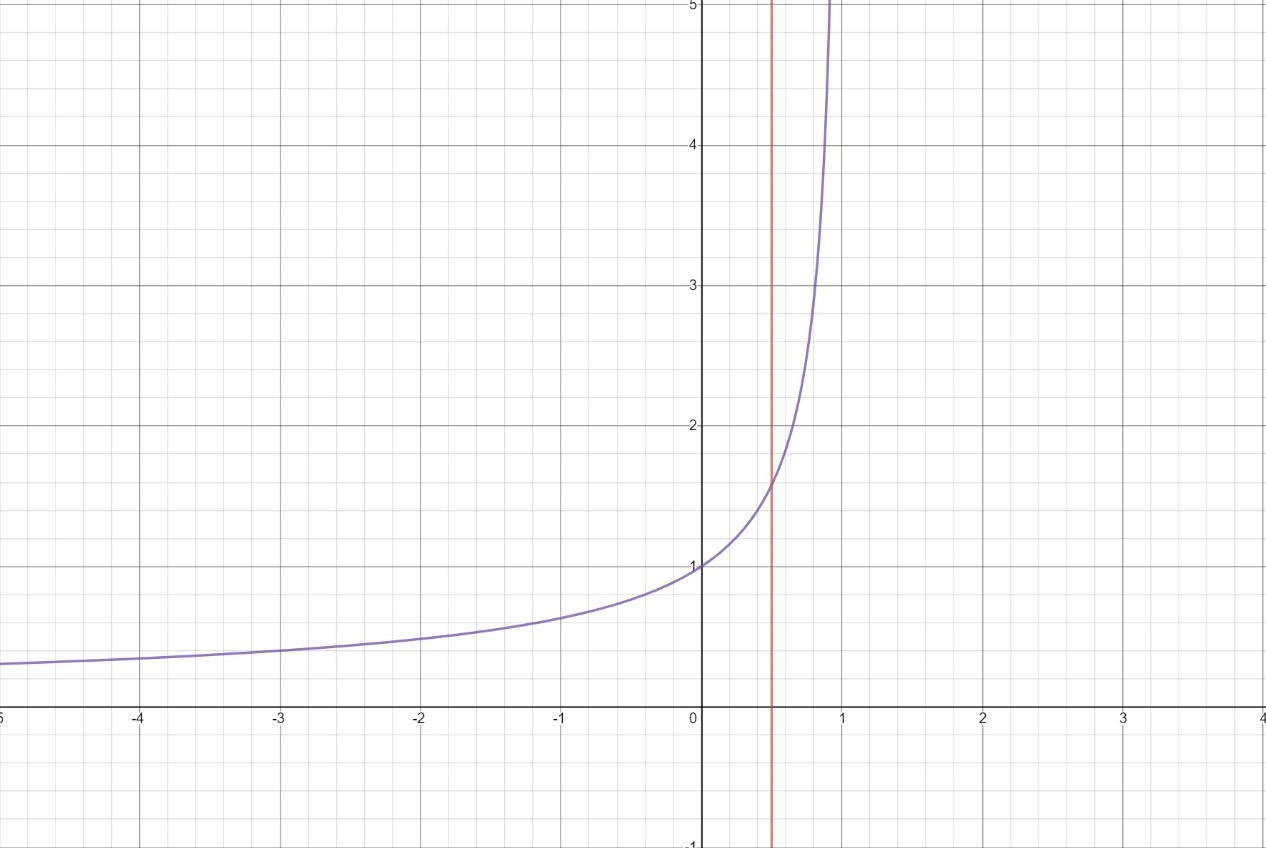
\includegraphics[width=60mm]{zeta-photo3.jpg}
     
    \end{center}
    \caption{\(Re(s)<1\)}
   
  \end{minipage}
  \begin{minipage}{0.5\hsize}
    \begin{center}
      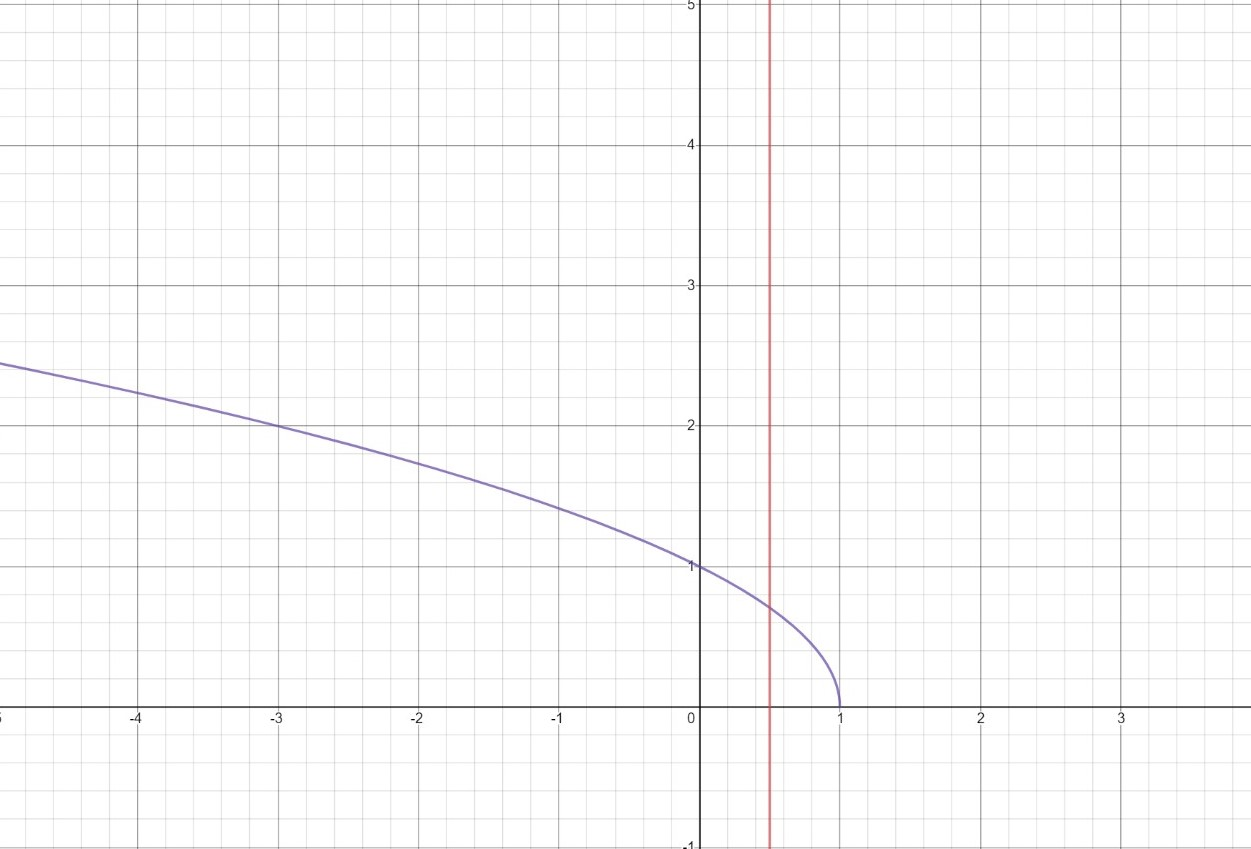
\includegraphics[width=60mm]{zeta-photo4.jpg}
    \end{center}
    \caption{\(Re(s)>1\)}
  \end{minipage}
\end{figure}
\\同様にして第二項について考える。\(\frac{1}{2}\leq x\leq1\)において\(x^{Re(t)-1}\)の最大値を\(C'\)と置けば、
\begin{align*}
\int_{\frac{1}{2}}^{1}(1-x)^{Re(s)-1}x^{Re(t)-1}dx&\leq C'\int_{\frac{1}{2}}^{1}(x-1)^{Re(s)-1}dx\\
&=C\left[\frac{(1-x)^{Re(s)}}{Re(s)}\right]_{\frac{1}{2}}^{1}=-\frac{C'}{2^{Re(s)}Re(s)}
\end{align*}
よって第二項は\(Re(s)>0\)で収束することが分かった。\\
以上よりベータ関数は\(Re(s)>0\)かつ、\(Re(t)>0\)で絶対収束する。\\
次に証明に移る。まず
\[\Gamma(s)\Gamma(t)=\left(\int_{0}^{\infty}e^{-x}x^{s-1}dx\right)\left(\int_{0}^{\infty}e^{-y}y^{t-1}dy\right)\]
であり、\(x=X^2,y=Y^2\)と変数変換すると、\(dx=2XdX,dy=2YdY\)であるから
\begin{align*}
\Gamma(s)\Gamma(t)&=\left(2\int_{0}^{\infty}e^{-X^2}X^{2s-2}XdX\right)\left(2\int_{0}^{\infty}e^{-Y^2}Y^{2t-2}YdY\right)\\
&=\left(2\int_{0}^{\infty}e^{-X^2}\frac{X^{2s-1}}{X}\cdot XdX\right)\left(2\int_{0}^{\infty}e^{-Y^2}\frac{Y^{2s-1}}{Y}\cdot XdX\right)\\
&=4\left(\int_{0}^{\infty}e^{-X^2}X^{2s-1}dX\right)\left(\int_{0}^{\infty}e^{-Y^2}Y^{2s-1}dY\right)\\
&=4\int_{0}^{\infty}\int_{0}^{\infty}e^{-(X^2+Y^2)}X^{2s-1}Y^{2t-1}dXdY
\end{align*}
最後の3行目から4行目の積分の順序変換はフビニの定理より保障される。\\
ここで\(X=r\cos\theta,\hspace{5mm}Y=r\sin\theta\)と変数変換すると、(\(0<r<\infty,0<\theta<2\pi\))
\begin{align}
\Gamma(s)\Gamma(t)&=4\int_{0}^{2}\pi\int_{0}^{\infty}e^{-r^2}(r\cos\theta)^{2s-1}(r\sin\theta)^{2t-1}rdrd\nonumber\theta\\
&=\left(2\int_{0}^{2\pi}(\cos\theta)^{2s-1}(\sin\theta)^{2t-1}d\theta\right)\left(2\int_{0}^{\infty}e^{-r^2}\cdot r^{2s-1}\cdot r^{2t-1}\cdot rdr\right)\nonumber\\
&=\left(2\int_{0}^{2\pi}(\cos\theta)^{2s-1}(\sin\theta)^{2t-1}d\theta\right)\left(2\int_{0}^{\infty}e^{-r^2}\cdot r^{2s+2t-1}dr\right)
\end{align}
これはヤコビアン
\[J=\frac{\partial(x,y)}{\partial(u,\upsilon)}=
\begin{vmatrix}
\frac{\partial x}{\partial u} & \frac{\partial x}{\partial\upsilon}\\
\frac{\partial y}{\partial u} & \frac{\partial y}{\partial\upsilon}\\
\end{vmatrix}
\]
に対し、\(f(x,y)\)を\(x=\phi(u,\upsilon),y=\psi(u,\upsilon)\)に変数変換するとき
\[\int\int_{D}f(x,y)dxdy=\int\int_{D'}f\left\{\phi(u,\upsilon),\psi(u,\upsilon)\right\}\left|J\right|dud\upsilon\]
であることを用いた。\\
(10)の式のうしろの積分について\(r^{2}=x\)と変数変換すると、\(2rdr=dx,\hspace{5mm}dr=\frac{dx}{2r}=\frac{dx}{2\sqrt{x}}\)であるから
\begin{align*}
2\int_{0}^{\infty}e^{-r^2}\cdot r^{2s+2t-1}dr&=2\int_{0}^{\infty}e^{-x}\left(x^{\frac{1}{2}}\right)^{2(s+t)-1}\frac{dx}{2\sqrt{x}}\\
&=\int_{0}^{\infty}e^{-x}x^{s+t-\frac{1}{2}}\frac{dx}{\sqrt{x}}\\
&=\int_{0}^{\infty}e^{-x}\cdot x^{\frac{1}{2}}\cdot x^{s+r-1}\frac{dx}{\sqrt{x}}=\int_{0}^{\infty}e^{-x}x^{s+t-1}dx=\Gamma(s+t)
\end{align*}
一方、ベータ関数
\[B(s,t)=\int_{0}^{1}(1-x)^{s-1}x^{t-1}sx\]
について、\(x=\sin^{2}\theta,\hspace{5mm}dx=2\sin\theta\cos\theta d\theta\)の置換より、
\begin{align*}
B(s,t)&=\int_{0}^{\frac{\pi}{2}}(1-\sin^{2}\theta)^{s-1}(\sin\theta)^{2(t-1)}\cdot2\sin\theta\cos\theta d\theta\\
&=2\int_{0}^{\frac{\pi}{2}}(\cos^{2}\theta)^{s-1}(\sin\theta)^{2t-1}\cos\theta d\theta\\
&=2\int_{0}^{\frac{\pi}{2}}(\cos\theta)^{2s-1}(\sin\theta)^{2t-1}d\theta
\end{align*}
よって(10)の式は
\[\Gamma(s)\Gamma(t)=B(s,t)\Gamma(s+t)\]
より証明された。\\
今度もルジャンドルの2倍公式を証明するために用いる以下の補題を証明する。\\
\\
<補題7.5>ガンマ関数の無限積表示1\\
\(\frac{1}{\Gamma(s)}\)は全平面で正則であり、以下の表示式をもつ。
\begin{equation}
\frac{1}{\Gamma(s)}=se^{\gamma s}\prod_{n=1}^{\infty}\left(1+\frac{s}{n}\right)e^{-\frac{s}{n}}
\end{equation}
〇証明\\
自然数\(N\)に対して次の関数を導入する。
\[
f_{N}(x)=\begin{cases}
\left(1-\frac{x}{N}\right)^{N} & (0<x<N)\\
0 & (x\geq N)\\
\end{cases}
\]
ベータ関数
\[B(s+N,t)=\int_{0}^{1}(1-x)^{s+N-1}x^{t-1}dx\]
を\(x\to\frac{x}{N}\)と置き換えると、(\(dx\to\frac{dx}{N},\hspace{5mm}x:0\to N\))
\begin{align*}
B(s+N,t)&=\int_{0}^{N}\left(1-\frac{x}{N}\right)^{s+N-1}\left(\frac{x}{N}\right)^{t-1}\frac{dx}{N}\\
&=\frac{1}{N^t}\int_{1}^{N}\left(1-\frac{x}{N}\right)^{N}\left(1-\frac{x}{N}\right)^{s-1}x^{t-1}dx\\
&=\frac{1}{N^t}\int_{0}^{N}f_{N}(x)\left(1-\frac{x}{N}\right)^{s-1}x^{t-1}dx
\end{align*}
となる。一方、左辺について先ほどの補題7.4より
\[B(s+N,t)=\frac{\Gamma(s+N)\Gamma(t)}{\Gamma(s+t+N)}\]
よって
\begin{equation}
\frac{\Gamma(s+N)\Gamma(t)}{\Gamma(s+t+N)}N^t=\int_{0}^{N}f_{N}(x)\left(1-\frac{x}{N}\right)^{s-1}x^{t-1}dx
\end{equation}
ここで\(f_{N}(x)\)について\(g(N)=\log f_{N}(x)\)と置き、\(N\)を実数\(t\)に拡張して
\begin{align*}
g(t)&=t\log\left(1-\frac{x}{t}\right)\\
g'(t)&=\log\left(1-\frac{x}{t}\right)+\frac{t}{1-\frac{x}{t}}\cdot-\frac{x}{t^2}\\
&=\log\left(1-\frac{x}{t}\right)+\frac{\frac{x}{t}}{1-\frac{x}{t}}
\end{align*}
\(\displaystyle\log(1-x)=-\sum_{n=1}^{\infty}\frac{x^{n}}{n},\hspace{10mm}\frac{a}{1-r}=\sum_{n-1}^{\infty}ar^{n-1}\)より、
\begin{align*}
g'(t)&=-\sum_{n=1}^{\infty}\frac{1}{n}\left(\frac{x}{t}\right)^{n}+\sum_{n=1}^{\infty}\left(\frac{x}{t}\right)^{n}\\
&=\sum_{n=1}^{\infty}\left(1-\frac{1}{n}\right)\left(\frac{x}{t}\right)^{n}\geq0
\end{align*}
よって\(g(t)\)は単調増加であり、\(f_{N}(x)\)も単調増加する。また、
\begin{align*}
\lim_{N\to\infty}\log f_{N}(x)+x&=\lim_{N\to\infty}N\log\left(1-\frac{x}{N}\right)+x\\
&=\lim_{N\to\infty}N\sum_{n=1}^{\infty}\frac{-1}{n}\left(\frac{x}{N}\right)^{n}+x\\
&=\lim_{N\to\infty}\left(-x+N\sum_{n=2}^{\infty}\frac{-1}{n}\left(\frac{x}{N}\right)^{n}\right)+x\\
&=\lim_{N\to\infty}N\sum_{n=2}^{\infty}\frac{-1}{n}\left(\frac{x}{N}\right)^{n}\\
&=-\lim_{N\to\infty}\left(\frac{x^2}{2N}+\frac{x^3}{3N}+\cdots\right)=0
\end{align*}
ゆえに
\[\lim_{N\to\infty}\log f_{N}(x)=-x,\hspace{15mm}\lim_{N\to\infty}f_{N}(x)=e^{-x}\]
となる。\(f_{N}(x)\)についてこれらを用いて式(12)の両辺に極限\(N\to\infty\)をとると
\begin{align*}
\lim_{N\to\infty}\frac{\Gamma(s+N)\Gamma(t)}{\Gamma(s+t+N)}N^t&=\lim_{N\to\infty}\int_{0}^{N}f_{N}(x)\left(1-\frac{x}{N}\right)^{s-1}x^{t-1}dx\\
&=\lim_{N\to\infty}\int_{0}^{N}e^{-x}x^{t-1}dx\\
&=\int_{0}^{\infty}e^{-x}x^{t-1}dx=\Gamma(t)
\end{align*}
となる。ここで1行目から2行目の極限のとり方はルベーク単調収束定理
\[\lim_{k\to\infty}\int f_{k}d\mu=\int\lim_{k\to\infty}f_{k}d\mu\]
を用いた。
よって
\[\lim_{N\to\infty}\frac{\Gamma(s+N)}{\Gamma(s+t+N)}N^{t}=1\]
\(s=1\)とすると
\[
\lim_{N\to\infty}\frac{N^{t}\cdot\Gamma(N+1)}{(t+N)(t+N-1)\cdots(t+1)t(t-1)(t-2)\cdots}
=1
\]
より
\[
\lim_{N\to\infty}\frac{N^{t}\cdot N!}{(t+N)(t+N-1)\cdots\Gamma(t)}=1
\]
両辺に\(\Gamma(t)\)を掛けて
\[\lim_{N\to\infty}\frac{N^{t}\cdot N!}{(t+N)(t+N-1)\cdots(t+1)t}=\Gamma(t)\]
これより
\begin{align*}
\frac{1}{\Gamma(t)}&=\lim_{N\to\infty}\frac{(t+N)(t+N-1)\cdots(t+1)t}{N^t\cdot N!}\\
&=\lim_{N\to\infty}N^{-t}\cdot\frac{(t+N)(t+N-1)\cdots(t+1)t}{N(N-1)(N-2)\cdots2\cdot1}\\
&=\lim_{N\to\infty}N^{-t}\cdot\left(\frac{t}{N}+1\right)\left(\frac{t}{N-1}+1\right)\cdots\left(\frac{t}{2}+1\right)\left(t+1\right)t\\
&=\lim_{N\to\infty}\left(e^{\log N}\right)^{-t}t\prod_{j=1}^{N}\left(\frac{t}{j}+1\right)\\
&=\lim_{N\to\infty}e^{-t\log N}t\prod_{j=1}^{N}\left(1+\frac{t}{j}\right)
\end{align*}
ここで\(\displaystyle1\left(=\prod_{j=1}^{N}e^{-\frac{t}{j}}\prod_{j=1}^{N}e^{\frac{t}{j}}\right)\)を掛けると
\begin{align*}
\frac{1}{\Gamma(t)}&=\lim_{N\to\infty}e^{-t\log N}t\prod_{j=1}^{N}\left(1+\frac{t}{j}\right)e^{-\frac{t}{j}}\prod_{j=1}^{N}e^{\frac{t}{j}}\\
&=\lim_{N\to\infty}\left(e^{-t\log N}\cdot e^{t+\frac{t}{2}+\frac{t}{3}\cdots}\right)t\prod_{j=1}^{N}\left(1+\frac{t}{j}\right)e^{-\frac{t}{j}}\\
&=\lim_{N\to\infty}e^{t\left(\sum_{t}^{N}\frac{1}{t}-\log N\right)}t\prod_{j=1}^{N}\left(1+\frac{t}{j}\right)e^{-\frac{t}{j}}\\
&=\lim_{N\to\infty}te^{\gamma t}\prod_{j=1}^{N}\left(1+\frac{t}{j}\right)e^{-\frac{t}{j}}
\end{align*}
最後の積の因子について、\(\displaystyle e^{x}=1+\sum_{n=1}^{\infty}\frac{x^{n}}{n!}\)であるから
\begin{align*}
\left(1+\frac{t}{j}\right)^{-\frac{t}{j}}&=\left(1+\frac{t}{j}\right)\left(1-\frac{t}{j}+O(j^{-2})\right)\\
&=1+O(j^{-2})
\end{align*}
より
\[\lim_{N\to\infty}\prod_{j=1}^{N}\left(1+\frac{t}{j}\right)e^{-\frac{t}{j}}\]
は収束する。以上より
\[
\frac{1}{\Gamma(t)}=se^{\gamma t}\prod_{j=1}^{\infty}\left(1+\frac{t}{j}\right)e^{-\frac{t}{j}}
\]
が成り立つ。また、この式からガンマ関数は\(t=-j(=0,1,2...)\)で一位の零点を持ち、それ以外の\(t\in\mathbb{C}\)で非零かつ正則であることが分かる。\\
さらに計算を進めてみる。この両辺の対数をとって計算していくと
\begin{align*}
-\log\Gamma(t)&=\log t+\gamma t+\log\left(\prod_{j=1}^{\infty}\left(1+\frac{t}{j}\right)e^{-\frac{t}{j}}\right)\\
&=\log t+\gamma t+\sum_{j=1}^{\infty}\log\left\{\left(1+\frac{t}{j}\right)e^{-\frac{t}{j}}\right\}\\
&=\log t+\gamma t+\sum_{j=1}^{\infty}\left\{\log\left(1+\frac{t}{j}\right)+\log e^{-\frac{t}{j}}\right\}\\
&=\log t+\gamma t+\sum_{j=1}^{\infty}\left\{\log\left(1+\frac{t}{j}\right)-\frac{t}{j}\right\}
\end{align*}
両辺を\(t\)で微分すると
\begin{align*}
-\frac{\Gamma'(t)}{\Gamma(t)}=\frac{1}{t}+\gamma+\sum_{j=1}^{\infty}\left(\frac{1}{1+\frac{t}{j}}-\frac{1}{j}\right)=\frac{1}{t}+\gamma+\sum_{j=1}^{\infty}\left(\frac{1}{j+t}-\frac{1}{j}\right)
\end{align*}
さらに両辺を微分すると
\[-\frac{d}{dt}\frac{\Gamma'(t)}{\Gamma(t)}=-\frac{1}{t^2}-\sum_{j=1}^{\infty}\frac{1}{(j+t)^2}\]
したがって
\begin{equation}
\frac{d}{dt}\frac{\Gamma'(t)}{\Gamma(t)}=\sum_{j=0}^{\infty}\frac{1}{(j+t)^{2}}
\end{equation}
を得る。
いよいよルジャンドルの二倍公式を証明する。\\
\\
<補題7.6>ルジャンドルの二倍公式\\
\begin{equation}
\Gamma(2s)=\frac{2^{2s-1}}{\sqrt{\pi}}\Gamma(s)\Gamma\left(s+\frac{1}{2}\right)
\end{equation}
〇証明\\
式(13)より、
\begin{align*}
\frac{d}{ds}\frac{\Gamma'(s)}{\Gamma(s)}+\frac{d}{ds}\frac{\Gamma'\left(s+\frac{1}{2}\right)}{\Gamma\left(s+\frac{1}{2}\right)}&=\sum_{n=0}^{\infty}\frac{1}{(n+s)^2}+\sum_{n=0}^{\infty}\frac{1}{\left(n+\frac{1}{2}+2s\right)^2}\\
&=4\left(\sum_{n=0}^{\infty}\frac{1}{(2n+2s)^2}+\sum_{n=0}^{\infty}\frac{1}{(2n+1+2s)^2}\right)\\
&=4\sum_{m=0}^{\infty}\frac{1}{(m+2s)^2}\\
\end{align*}
ここで前補題の証明過程より
\[-\frac{\Gamma'(as)}{\Gamma(as)}=\frac{1}{as}+\gamma+\sum_{n=1}^{\infty}\left(\frac{1}{n+as}-\frac{1}{n}\right)\]
を微分すると
\[-\frac{d}{ds}\frac{\Gamma'(as)}{\Gamma(as)}=-\frac{1}{as^2}-a\sum_{n=1}^{\infty}\frac{1}{(n+as)^2}=-a\sum_{n=0}^{\infty}\frac{1}{(n+as)^2}\]
であるから
\[\frac{d}{ds}\frac{\Gamma'(s)}{\Gamma(s)}+\frac{d}{ds}\frac{\Gamma'\left(s+\frac{1}{2}\right)}{\Gamma\left(s+\frac{1}{2}\right)}=2\frac{d}{ds}\frac{\Gamma'(2s)}{\Gamma(2s)}\]
であり、両辺を一度積分すると
\[\frac{\Gamma'(s)}{\Gamma(s)}+C_{1}+\frac{\Gamma'\left(s+\frac{1}{2}\right)}{\Gamma\left(s+\frac{1}{2}\right)}+C_{2}=2\frac{\Gamma'(2s)}{\Gamma(2s)}+C_{3}\]
となる。さらに両辺を積分すると
\[\log\Gamma(s)+C'_{1}+sC_{1}+\log\Gamma\left(s+\frac{1}{2}\right)+C'_{2}+sC_{2}=2\log\Gamma(2s)+C'_{3}+sC_{3}\]
定数をまとめて整理すると
\begin{align*}
\log\Gamma(s)+\Gamma\left(s+\frac{1}{2}\right)&=as+b+2\log\Gamma(2s)\\
\log\left(\Gamma(s)\Gamma\left(s+\frac{1}{2}\right)\right)&=\log\left(e^{as+b'}\Gamma(2s)\right)
\end{align*}
となり、対数をとると
\[\Gamma(s)\Gamma\left(s+\frac{1}{2}\right)=e^{as+b'}\Gamma(2s)\]
となる。\(s=\frac{1}{2}\)を代入すると
\[\Gamma\left(\frac{1}{2}\right)\Gamma(1)=e^{\frac{a}{2}+b'}\Gamma(1)\]
一方、\(s=1\)を代入すると
\[\Gamma(1)\Gamma\left(1+\frac{1}{2}\right)=e^{a+b'}\Gamma(2)\]
であり、\(\Gamma(1)=\Gamma(2)=1\),\(\Gamma\left(\frac{1}{2}\right)=\sqrt{\pi}\).また、\(\Gamma(s+1)=s\Gamma(s)\)より、\(\Gamma\left(1+\frac{1}{2}\right)=\frac{\Gamma\left(\frac{1}{2}\right)}{2}=\frac{\sqrt{\pi}}{2}\)であるから、これらを代入するとそれぞれ
\begin{align*}
\sqrt{\pi}=e^{\frac{a}{2}+b'}&\Longleftrightarrow\frac{1}{2}\log\pi=\frac{a}{2}+b'\\
\frac{\sqrt{\pi}}{2}=e^{a+b'}&\Longleftrightarrow\frac{1}{2}\log\pi-\log2=a+b'
\end{align*}
以上より
\[a=-\log2,\hspace{15mm}b=\frac{1}{2}\log\pi+\log2\]
と求まり、証明完了。\\
<補題7.7>ガンマ関数の無限乗積表示2\\
\begin{equation}
\Gamma(z)=\lim_{n\to\infty}\frac{n^{z}n!}{\prod_{k=0}^{n}(z+k)}
\end{equation}
〇証明\\
\[G_{n}(z)=\int_{0}^{n}t^{z-1}\left(1-\frac{t}{n}\right)^{n}dt\]
とすれば
\[\lim_{n\to\infty}G_{n}(z)=\int_{0}^{\infty}t^{z-1}e^{-t}dt=\Gamma(z)\]
である。\(G_{n}(z)\)について、\(t=nu\)と置換すれば、(\(dt=ndu,\hspace{5mm}t:0\to n,\hspace{5mm}u:0\to1\))
\begin{align*}
G_{n}(z)&=\int_{0}^{1}(nu)^{z-1}(1-u)^{n}\cdot ndu\\
&=n^{z}\int_{0}^{1}u^{z-1}(1-u)^{n}du
\end{align*}
ここで\(\displaystyle I_{n}(z)=\int_{0}^{1}u^{z-1}(1-u)^{n}du\)とおくと
\begin{align*}
I_{n}(z)&=\int_{0}^{1}\left(\frac{u^{z}}{z}\right)'(1-u)^{n}du=\Biggl[\frac{u^{z}}{x}(1-u)^{n}\Biggr]_{0}^{1}-\int_{0}^{1}\frac{u^{z}}{z}(-n)(1-u)^{n-1}du\\
&=0+\frac{n}{z}\int_{0}^{1}u^{z}(1-u)^{n-1}du
\end{align*}
よって
\[I_{n}(z)=\frac{n}{z}I_{n-1}(z+1)\]
であるから、
\[I_{n}(z)=\frac{n!}{\prod_{k=0}^{n}(z+k)}\]
\[G_{n}(z)=n^{z}I_{n}=\frac{n^{z}n!}{\prod_{k=0}^{n}(z+k)}\]
これより極限をとれば示される。この式は一般の複素数について成り立っている。\\
\\
これを用いてオイラーの相反公式を証明する。\\
<補題7.8>オイラーの相反公式\\
ガンマ関数についての関数等式
\begin{equation}
\Gamma(z)\Gamma(1-z)=\frac{\pi}{\sin\pi z}
が成り立つ。
\end{equation}
まず\(\Gamma(1+z)=z\Gamma(z)\)より
\[\Gamma(z)\Gamma(1-z)=-z\Gamma(z)\Gamma(-z)\]
これよりガンマ関数の無限乗積表示を代入すれば
\begin{align*}
-z\Gamma(z)\Gamma(-z)&=-z\left(\lim_{n\to\infty}\frac{n^{z}n!}{\prod_{k=0}^{n}(z+k)}\right)\left(\lim_{n\to\infty}\frac{n^{-z}n!}{\prod_{k=0}^{n}(-z+k)}\right)\\
&=-z\lim_{n\to\infty}\frac{n!n!}{\prod_{k=0}^{n}(k^{2}-z^{2})}\\
&=-z\cdot\frac{1}{-z^2}\lim_{n\to\infty}\frac{n!n!}{\prod_{k=1}^{n}(k^{2}-z^{2})}\\
&=\frac{1}{z}\prod_{k=1}^{\infty}\frac{k^2}{k^{2}-z^{2}}=\frac{\pi}{\pi z\prod_{k=1}^{\infty}\frac{k^{2}-z^{2}}{k^{2}}}
\end{align*}
ここで
\[\sin\pi z=\pi z\prod_{n=1}^{\infty}\left(1-\frac{z^2}{n^{2}}\right)\]
より
\[-z\Gamma(z)\Gamma(-z)=\frac{\pi}{\sin\pi z}\]
より証明された。







\setcounter{equation}{0}
\section{特殊値}
ゼータ関数の変数sが整数であるような、特別な場合に成り立つ2式を証明する。\\
<定理8.1>\\
正整数\(k\)に対して
\begin{equation}
\zeta(2k)=(-1)^{k+1}\frac{(2\pi)^{2k}B_{2k}}{2(2k)!}
\end{equation}
\\
<定理8.2>\\
自然数\(k\)に対して
\begin{equation}
\zeta(-k)=(-1)^{k}\frac{B_{k+1}}{k+1}
\end{equation}
\begin{equation}
\zeta(1-2k)=-\frac{B_{2k}}{2k}
\end{equation}
\\
\\
以上の定理の証明に移る前にそれに用いる補題を証明しておく。\\
\\
<補題8.3>ガンマ関数の極における留数\\
\(\Gamma(s)\)の\(s=-n(n\in\mathbb{N})\)の一位の極における留数は\(\displaystyle\frac{(-1)^{n}}{n!}\)である。\\
〇証明\\
点\(a\)が関数\(f(z)\)の1位の極であるとき、その留数は
\[Res[f,a]=\lim_{z\to a}(z-a)f(z)\]
であるから、ガンマ関数の留数は
\begin{align*}
\lim_{s\to-n}(s+n)\Gamma(s)&=\lim_{s\to-n}(s+n)\frac{\Gamma(s+1)}{s}\hspace{10mm}\left(\because\Gamma(s+1)=s\Gamma(s)\right)\\
&=\lim_{s\to-n}(s+n)\frac{\Gamma(s+2)}{s(s+1)}\\
\end{align*}
以降繰り返すことで
\begin{align*}
&=\cdots\\
&=\lim_{s\to-n}(s+n)\frac{\Gamma(s+n+1)}{s(s+1)(s+2)\cdots(s+n)}\\
&=\lim_{s\to-n}\frac{\Gamma(s+n+1)}{s(s+1)\cdots(s+n-1)}\\
&=\frac{\Gamma(1)}{-n(-n+1)\cdots(-1)}=\frac{(-1)^{n}}{n!}
\end{align*}
より証明完了。\\
定理8.1の証明に移る。\\
〇証明(8.1)\\
正弦関数の無限乗積表示
\[\sin x=x\prod_{r=1}^{\infty}\left(1-\frac{x^{2}}{\pi^{2}r^{2}}\right)\]
から始める。\(x=\frac{u}{2i}\)と置くと、\(\sin x=\frac{e^{ix}-e^{-ix}}{2i}\)より左辺は
\[\sin\frac{u}{2i}=\frac{e^{\frac{u}{2}}-e^{-\frac{u}{2}}}{2i}=\frac{e^{\frac{u}{2}}\left(1-e^{-u}\right)}{2i}\]
右辺は
\begin{align*}
\frac{u}{2i}\prod_{r=1}^{\infty}\left(1-\frac{1}{\pi^{2}r^{2}}\left(-\frac{u^2}{4}\right)\right)&=\frac{u}{2i}\prod_{r=1}^{\infty}\left(1+\frac{u^2}{4\pi^{2}r^{2}}\right)\\
&=\frac{u}{2i}\prod_{r=1}^{\infty}\left(\frac{4\pi^{2}r^{2}+u^{2}}{4\pi^{2}r^{2}}\right)
\end{align*}
であるから
\[\frac{e^{\frac{u}{2}}\left(1-e^{-u}\right)}{2i}=\frac{u}{2i}\prod_{r=1}^{\infty}\left(\frac{4\pi^{2}r^{2}+u^{2}}{4\pi^{2}r^{2}}\right)\]
両辺の対数をとると
\[\log e^{\frac{u}{2}}+\log(1-e^{-u})-\log2i=\log u-\log2i+\sum_{r=1}^{\infty}\log\left(\frac{4\pi^{2}r^{2}+u^{2}}{4\pi^{2}r^{2}}\right)\]
両辺を微分すると
\[\frac{1}{2}+\frac{e^{-u}}{1-e^{-u}}=\frac{1}{u}+\sum_{r=1}^{\infty}\left(\frac{2u}{4\pi^{2}r^{2}}\cdot\frac{4\pi^{2}r^{2}}{4\pi^{2}r^{2}+u^2}\right)\]
よって
\[\frac{1}{2}+\frac{1}{e^{u}-1}=\frac{1}{u}+\sum_{r=1}^{\infty}\frac{2u}{4\pi^{2}r^{2}+u^2}\]
ここでベルヌーイ数の定義
\[f(x)=\frac{x}{e^{x}-1}=\sum_{n=0}^{\infty}\frac{B_{n}}{n!}x^n\]
より
\[\frac{1}{e^{u}-1}=\frac{1}{u}\sum_{k=0}^{\infty}\frac{B_{k}}{k!}u^{k}\]
であるから左辺について
\begin{align*}
\frac{1}{2}+\frac{1}{e^{u}-1}&=\frac{1}{2}+\frac{1}{u}\sum_{k=0}^{\infty}\frac{B_{k}}{k!}u^{k}\\
&=\frac{1}{2}+\left(\frac{1}{u}\cdot\frac{B_{0}}{0!}\right)+\left(\frac{1}{u}\cdot\frac{B_{1}}{1!}u\right)+\frac{1}{u}\sum_{k=2}^{\infty}\frac{B_{k}}{k!}u^{k}\\
&=\frac{1}{2}+\frac{1}{u}-\frac{1}{2}+\frac{1}{u}\sum_{k=2}^{\infty}\frac{B_{k}}{k!}u^{k}
\end{align*}
ゆえに
\[\frac{1}{2}+\frac{1}{u}-\frac{1}{2}+\frac{1}{u}\sum_{k=2}^{\infty}\frac{B_{k}}{k!}u^{k}=\frac{1}{u}+\sum_{r=1}^{\infty}\frac{2u}{4\pi^{2}r^{2}+u^2}\]
これより
\begin{align*}
\sum_{k=2}^{\infty}\frac{B_{k}}{k!}u^{k}&=u\sum_{r=1}^{\infty}\frac{2u}{4\pi^{2}r^{2}+u^2}=2\sum_{r=1}^{\infty}\frac{u^2}{4\pi^{2}r^{2}+u^2}\\
&=2\sum_{r=1}^{\infty}\left(\frac{u}{2\pi r}\right)^2\cdot\frac{(2\pi r)^2}{4\pi^{2}r^{2}+u^2}=s\sum_{r=1}^{\infty}\left(\frac{u}{2\pi r}\right)^2\frac{1}{1+\left(\frac{u}{2\pi r}\right)^2}
\end{align*}
ここで\(\displaystyle\frac{1}{1+\left(\frac{u}{2\pi r}\right)^2}=\frac{1}{1-\left(-\left(\frac{u}{2\pi r}\right)^2\right)}\)と考えて無限和の公式\(\displaystyle\frac{a}{1-r}=\sum_{n=1}^{\infty}ar^{n-1}\)を使うと
\[\frac{1}{1+\left(\frac{u}{2\pi r}\right)^2}=\sum_{n=1}^{\infty}\left\{-\left(\frac{u}{2\pi r}\right)^2\right\}^{n-1}=\sum_{n=0}^{\infty}(-1)^{n}\left(\frac{u}{2\pi r}\right)^{2n}\]
となる。よって
\begin{align*}
\sum_{k=2}^{\infty}\frac{B_{k}}{k!}u^{k}&=2\sum_{r-1}^{\infty}\left(\frac{u}{2\pi r}\right)^{2}\sum_{n=0}^{\infty}(-1)^{n}\left(\frac{u}{2\pi r}\right)^{2n}\\
&=2\sum_{n=0}^{\infty}(-1)^{n}\sum_{r=1}^{\infty}\left(\frac{u}{2\pi r}\right)^{2n+2}\\
&=2\sum_{n=1}^{\infty}(-1)^{n+1}\sum_{r=1}^{\infty}\left(\frac{u}{2\pi r}\right)^{2n}\\
&=2\sum_{n=1}^{\infty}(-1)^{n+1}\cdot\frac{u^{2n}}{(2\pi)^{2n}}\sum_{r=1}^{\infty}\frac{1}{r^{2n}}\\
&=2\sum_{n=1}^{\infty}\left((-1)^{n+1}\cdot\frac{\zeta(2n)}{(2\pi)^{2n}}\right)u^{2n}
\end{align*}
両辺の\(u^{2n}\)について係数比較することにより
\[\frac{B_{2n}}{(2n)!}=2(-1)^{n+1}\cdot\frac{\zeta(2n)}{(2\pi)^{2n}}\]
より定理の式を得る。次に定理8.2を証明する。\\
〇証明(8.2)\\
ゼータ関数の積分表示
\[\zeta(s)=\frac{1}{\Gamma(s)}\int_{0}^{\infty}\frac{x^{s-1}}{e^{x}-1}dx\]
より
\begin{align*}
\zeta(s)&=\frac{1}{\Gamma(s)}\int_{1}^{\infty}\frac{x^{s-1}}{e^{x}-1}dx+\frac{1}{\Gamma(s)}\int_{0}^{1}\frac{x^{s-1}}{e^{x}-1}dx\\
&=\frac{1}{\Gamma(s)}\int_{1}^{\infty}\frac{x^{s-1}}{e^{x}-1}dx+\frac{1}{\Gamma(s)}\int_{0}^{1}x^{s-2}\frac{x}{e^{x}-1}dx\\
&=\frac{1}{\Gamma(s)}\int_{1}^{\infty}\frac{x^{s-1}}{e^{x}-1}dx+\frac{1}{\Gamma(s)}\int_{0}^{1}x^{s-2}\left(\frac{x}{e^{x}-1}-\sum_{n=0}^{K}\frac{B_{n}}{n!}x^{n}\right)dx+\frac{1}{\Gamma(s)}\int_{0}^{1}x^{s-2}\sum_{n=0}^{K}\frac{B_{n}}{n!}x^{n}dx
\end{align*}
ここで\(K\)は\(K>m\)を満たす定数で有限和をとる。
\begin{align*}
I_{1}(s)&=\int_{1}^{\infty}\frac{x^{s-1}}{e^{x}-1}dx\\
I_{2}(s)&=\int_{0}^{1}x^{s-2}\left(\frac{x}{e^{x}-1}-\sum_{k=0}^{K}\frac{B_{k}}{k!}x^{k}\right)dx\\
I_{3}(s)&=\int_{0}^{1}x^{s-2}\sum_{k=0}^{K}\frac{B_{k}}{k!}x^{k}dx
\end{align*}
とおくと
\[\zeta(s)=\frac{I_{1}(s)}{\Gamma(s)}+\frac{I_{2}(s)}{\Gamma(s)}+\frac{I_{3}(s)}{\Gamma(s)}\]
と書ける。ここで\(I_{1}(s)\)は任意の\(s\in\mathbb{C}\)で正則で\(I_{2}(s)\)は\(Re(s)>-K\)で正則である(ともに有限値をとる)から、ガンマ関数の零点の影響で
\[\lim_{s\to-m}\frac{I_{1}(s)}{\Gamma(s)}=0\]
\[\lim_{s\to-m}\frac{I_{2}(s)}{\Gamma(s)}=0\]
となる。\(I_{2}(s)\)が\(Re(s)>-K\)で有限値をとることは
\[\frac{x}{e^{x}-1}-\sum_{k=0}^{K}\frac{B_{k}}{k!}x^{k}=O(x^{K+1})\hspace{5mm}(0<x<1)\]
であることより分かる。以上より\(\zeta(s)\)の極限\(s\to-m\)を考えるときは、第三項目のみ考えればよい。\(I_{3}(s)\)について
\begin{align*}
I_{3}(s)&=\int_{0}^{1}x^{s-2}\sum_{k=0}^{K}\frac{B_{k}}{k!}x^{k}dx
=\sum_{k=0}^{K}\frac{B_{k}}{k!}\int_{0}^{1}x^{s+k-2}dx\\
&=\sum_{k=0}^{K}\frac{B_{k}}{k!}\Biggl[\frac{x^{s+k-1}}{s+k-1}\Biggr]_{0}^{1}
=\sum_{k=0}^{K}\frac{B_{k}}{k!}\cdot\frac{1}{s+k-1}
\end{align*}
となり、\(k=0,1,...\)に対して
\[I_{3}(s)=\frac{B_{1}}{0!}\frac{1}{s-1}+\frac{B_{1}}{1!}\frac{1}{s}+\cdots+\frac{B_{m}}{m!}\frac{1}{s+m-1}+\frac{B_{m+1}}{(m+1)!}\frac{1}{s+m}+\frac{B_{m+2}}{(m+2)!}\frac{1}{s+m+1}+\cdots\]
であるので\(s\to-m\)を考えたとき、途中の\(k=m+1\)の項以外は有界である。ゆえに\(\displaystyle\lim_{s\to-m}\frac{I_{3}(s)}{\Gamma(s)}\)を考えるとき、\(k=m+1\)の項だけを取り出して\(I_{3}(s)\to\frac{B_{n+1}}{(m+1)!}\cdot\frac{1}{s+m}\)と考えてよい。(他の項はガンマ関数の零点によって消える。)したがって
\begin{align*}
\lim_{s\to-m}\zeta(s)=\zeta(-m)&=0+0+\lim_{s\to-m}\frac{I_{3}(s)}{\Gamma(s)}\\
&=\lim_{s\to-m}\frac{1}{(s+m)\Gamma(s)}\cdot(s+m)I_{3}(s)\\
&=\lim_{s\to-m}\frac{1}{(s+m)\Gamma(s)}\cdot\frac{B_{m+1}}{(m+1)!}=\frac{1}{Res_{s=-m}\Gamma(s)}\cdot\frac{B_{m+1}}{(m+1)!}\\
&=\frac{m!}{(-1)^{m}}\cdot\frac{B_{m+1}}{(m+1)!}\\
&=(-1)^{m}\cdot\frac{B_{m+1}}{m+1}
\end{align*}
より証明された。








\setcounter{equation}{0}
\section{アダマール積表示}
ゼータ関数のアダマール積表示について述べる。\\
<定理9.1>アダマール積表示\\
ゼータ関数の完備化\(\xi(s)=s(1-s)\hat{\zeta}(s)\)のアダマール積は
\begin{equation}
\xi(s)=-e^{as}\prod_{\rho}\left(1-\frac{s}{\rho}\right)e^{\frac{s}{\rho}}
\end{equation}
と書ける。ここで\(\rho\)は\(\zeta(s)\)の非自明零点であり、定数\(a\)は
\[a=\log2+\frac{1}{2}\log\pi-1-\frac{1}{2}\gamma\]である。\\
この定理を証明する前に完備ゼータ関数の位数について述べる。\\
\\
<補題9.2>完備ゼータの位数\\
正関数\(\xi(s)=s(1-s)\hat{\zeta}(s)\)の位数は1である。\\
〇証明\\
まず始めに\(\xi(s)\)の位数が1以下であることを示す。\\
\(\xi(s)=\xi(1-s)\)より\(Re(s)\geq\frac{1}{2}\)で\(|\xi(s)|\)を評価すれば十分である。\\
スターリングの公式
\begin{equation}
\Gamma(s)\sim\sqrt{2\pi}s^{s-\frac{1}{2}}e^{-s}\hspace{8mm}(|s|\to\infty)
\end{equation}
より\(s=\sigma\in\mathbb{R}\)のとき
\begin{align*}
\Gamma(\sigma)\sim\sqrt{2\pi}\sigma^{\sigma-\frac{1}{2}}e^{-\sigma}&=\sqrt{2\pi}e^{\left(\sigma-\frac{1}{2}\right)\log\sigma}e^{-\sigma}\\
&=\sqrt{2\pi}e^{\sigma\log\sigma-\frac{1}{2}\log\sigma-\sigma}=O\left(e^{\sigma\log\sigma}\right)\hspace{5mm}(\sigma\to\infty)
\end{align*}
これより
\begin{align*}
\left|\Gamma\left(\frac{s}{2}\right)\right|&=\left|\int_{0}^{\infty}e^{-u}u^{\frac{s}{2}-1}du\right|\\
&\leq\int_{0}^{infty}e^{-u}u^{\frac{\sigma}{2}-1}du\hspace{5mm}(Re(s)=\sigma)\\
&=\Gamma\left(\frac{\sigma}{2}\right)=O\left(e^{\frac{\sigma}{2}\log\frac{\sigma}{2}}\right)=O\left(e^{\frac{\sigma}{2}\log\sigma}\right)=O\left(e^{\frac{1}{2}|s|\log|s|}\right)\hspace{5mm}(\sigma<|s|)
\end{align*}
という評価が成り立つ。また、\(\zeta(s)\)について定理5.2より
\[\zeta(s)=\frac{1}{2}+\frac{1}{1-s}-s\int_{0}^{\infty}\frac{x-[x]-\frac{1}{2}}{x^{s+1}}dx\]
と表され、\(-\frac{1}{2}\leq x-[x]-\frac{1}{2}<1\)であるから、\(\sigma\geq\frac{1}{2}\)ならば
\[\zeta(s)=O\left(|s|\int_{0}^{\infty}\frac{1}{x^{\frac{3}{2}}}dx\right)=O(|s|)\hspace{5mm}(|s|\to\infty)\]
以上より
\[\xi(s)=s(1-s)\hat{\zeta}(s)=s(1-s)\pi^{-\frac{s}{2}}\Gamma\left(\frac{s}{2}\right)\zeta(s)\]
で
\[\lim_{s\to\infty}s(1-s)\pi^{-\frac{s}{2}}=0\]
より
\begin{align*}
\xi(s)&=O\left(e^{\log|s|}e^{\frac{1}{2}|s|\log|s|}\right)\\
&=O\left(e^{\frac{1}{2}|s|\log|s|+\log|s|}\right)=O\left(e^{\left(\frac{1}{2}+\frac{1}{|s|}\right)|s|\log|s|}\right)
\end{align*}
ゆえに、任意の\(\epsilon>0\)と\(\sigma\geq\frac{1}{2}\)に対して
\[\xi(s)=O\left(e^{\left(\frac{1}{2}+\epsilon\right)|s|\log|s|}\right)\hspace{10mm}(|s|\to\infty)\]
位数は任意の\(\epsilon>0\)に対して、十分大きな\(r\)を用いて
\[\max_{|s|=r}|f(s)|\leq e^{r^{\lambda+\epsilon}}\]
が成り立つような最小の数\(\lambda\)であるから先ほどの式に当てはめると
\[e^{\left(\frac{1}{2}+\epsilon\right)|r|\log|r|}\leq e^{r^{\lambda+\epsilon}}\]
が成り立つような最小の\(\lambda\)が位数である。これは\(\lambda=1\)である。\\
したがって\(\xi(s)\)の位数が1以下であることが分かった。\\
次に\(\xi(s)\)の位数が1以上であることを示す。スターリングの公式より、\(s=\sigma\in\mathbb{R}\)のとき
\begin{align*}
\Gamma\left(\frac{s}{2}\right)=\Gamma\left(\frac{\sigma}{2}\right)&\sim\sqrt{2\pi}\left(\frac{\sigma}{2}\right)^{\left(\frac{\sigma}{2}-\frac{1}{2}\right)}e^{-\frac{\sigma}{2}}\\
&=\sqrt{2\pi}e^{\left(\frac{\sigma}{2}-\frac{1}{2}\right)\log\frac{\sigma}{2}-\frac{\sigma}{2}}=\sqrt{2\pi}e^{\frac{1}{2}\left(\sigma-1\right)\log\frac{\sigma}{2}-\frac{\sigma}{2}}\hspace{10mm}(s=\sigma\to\infty)
\end{align*}
となる。\(\zeta(s)\)については4章の式(2)より
\begin{align*}
\log\zeta(s)&=\sum_{p:素数}\sum_{m=1}^{\infty}\frac{1}{mp^{ms}}\\
&=\sum_{p}\left(\frac{1}{p^s}+\frac{1}{2p^{2s}}+\frac{1}{3p^{3s}}+\cdots\right)
\end{align*}
であるから展開したときの第一項のみ残し、近似すると
\[\log\zeta(s)\sim2^{-s}\hspace{10mm}(s=\sigma\to\infty)\]
以上より\(s\in\mathbb{R}\)のとき、
\[\log|\xi(s)|\sim\frac{1}{2}s\log s\hspace{10mm}(s\to\infty)\]
となるので、\(\xi(s)\)の位数は最低でも1である。\\
以上より\(\xi(s)\)の位数はちょうど1である。\\
\\
定理9.1の証明に移る。\\
〇証明(9.1)\\
\(\xi(s)\)は\(s=1\)において因数\((1-s)\)と\(\zeta(s)\)の\(s=1\)が打ち消し合うので非零正則である。\\
\(\zeta(s)\)の自明零点\(s\)の位数が2以上であるとすると、\(\frac{s}{2}\)においてガンマ関数は1位の極をもつので位数が一致せず
\[\hat{\zeta}(1-s)=\hat{\zeta}(s)=\pi^{-\frac{s}{2}}\Gamma\left(\frac{s}{2}\right)\zeta(s)\]
の右辺が0になってしまう。しかし、左辺の\(\hat{\zeta}(s)\)は\(Re(1-s)>1\)で非零なので矛盾してしまう。よって\(\zeta(s)\)の自明零点の位数は1である。ガンマ関数の極と打ち消し合う。\\
また、\(\xi(s)\)の因数\(s\)について\(s=0\)のとき、ガンマ関数の1位の極と打ち消し合うのでやはり、\(s=0\)でも非零正則である。\\
以上より\(\xi(s)\)の零点は\(\zeta(s)\)の非自明零点であることが分かった。\(\xi(s)\)は整関数で位数が1であるから、アダマールの因数分解定理より
\[\xi(s)=Ce^{as}\prod_{\rho}\left(1-\frac{s}{\rho}\right)e^{\frac{s}{\rho}}\]
で表すことができる。定数\(C,a\)を求める。









\setcounter{equation}{0}
\section{素数分布}
\noindent
<定理10.1>\\
ある正の定数\(C_{1},C_{2}\)が存在し、任意の\(x\geq2\)に対して次の不等式が成り立つ。
\begin{equation}
C_{2}\frac{x}{\log x}\leq\pi(x)\leq C_{1}\frac{x}{\log x}
\end{equation}
\\
<定理10.2>\\
\(n\)番目の素数を\(p_{n}\)とする。ある正の定数\(D_{1},D_{2}\)が存在して、任意の\(n\)に対して次の不等式が成り立つ。
\begin{equation}
D_{2}n\log n\leq p_{n}\leq D_{1}n\log n
\end{equation}
\\
<定理10.3>\\
\(p\)を素数とすると
\begin{equation}
\sum_{p\leq x}\frac{\log p}{p}=\log x+O(1)
\end{equation}
\\
<定理10.4>\\
\(p\)を素数とすると
\begin{equation}
\sum_{p\leq n}\frac{\log p}{p}>\log n-3
\end{equation}
\\
<定理10.5>\\
素数\(p\)とある定数\(a\)に対して
\begin{equation}
\sum_{p\leq x}\frac{1}{p}=\log\log x+a+O\left(\frac{1}{\log x}\right)
\end{equation}
\\
<定理10.6>\\
ある定数\(C\)が存在して、次式が成り立つ。
\begin{equation}
\prod_{p\leq x}\left(1-\frac{1}{p}\right)\sim\frac{C}{\log x}
\end{equation}
\\
<定理10.7>\\
\newpage
〇証明(10.1)\\
まず\(x\geq 2\)と任意の\(0<\epsilon<1\)に対し
\[\theta(x)=\sum_{p\leq x}\log p\geq\sum_{x^{1-\epsilon}<p\leq x}\log p\]
である。また、\(x^{1-\epsilon}<p\)より
\[\sum_{x^{1-\epsilon}<p\leq x}\log p\geq\sum_{x^{1-\epsilon}<p\leq x}\log x^{1-\epsilon}=\log x^{1-\epsilon}\sum_{x^{1-\epsilon}<p\leq x}1\]
ここで
\[\sum_{x^{1-\epsilon}<p\leq x}1=\pi(x)-\pi(x^{1-\epsilon})\]
より
\begin{align*}
\theta(x)=\sum_{p\leq x}\log p&\geq\left(\pi(x)-\pi(x^{1-\epsilon})\right)\log x^{1-\epsilon}\\
&=\left(\pi(x)-\pi(x^{1-\epsilon})\right)(1-\epsilon)\log x
\end{align*}
また、
\[\pi(x^{1-\epsilon})\leq x^{1-\epsilon}\]
であるから
\begin{align*}
\theta(x)&\geq\left(\pi(x)-x^{1-\epsilon}\right)(1-\epsilon)\log x\\
&=\pi(x)(1-\epsilon)\log x-x^{1-\epsilon}(1-\epsilon)\log x
\end{align*}
\[\theta(x)+x^{1-\epsilon}(1-\epsilon)\log x\geq\pi(x)(1-\epsilon)\log x\]
より
\[\pi(x)\leq\frac{1}{1-\epsilon}\frac{\theta(x)}{\log x}+x^{1-\epsilon}\]
一方、
\[\theta(x)=\sum_{p\leq x}\log p\leq\sum_{p\leq x}\log x=\pi(x)\log x\]
より
\[\frac{\theta(x)}{\log x}\leq\pi(x)\]
であるから、さっきの結果と合わせて
\[\frac{\theta(x)}{\log x}\leq\pi(x)\leq\frac{1}{1-\epsilon}\frac{\theta(x)}{\log x}+x^{1-\epsilon}\]
ここで\(\frac{\log x}{x^\epsilon}\)は微分して分かるように極大値があり、また上に有界である。したがって正の定数で\(\frac{\log x}{x^{\epsilon}}\leq C\)と上から抑えられる。両辺に\(x\)を掛けて左辺をまとめると\(x^{1-\epsilon}\leq C\frac{x}{\log x}\)となる。また、前回の結果より定数\(A=1.1224\)を用いて\(\theta(x)\leq A_{1}x\)とできる。これらに置き換えることにより
\[\frac{A_{1}x}{\log x}\leq\pi(x)\leq\frac{1}{1-\epsilon}\frac{A_{1}x}{\log x}+C\frac{x}{\log x}\]
\[A_{1}\frac{x}{\log x}\leq\pi(x)\leq\left(\frac{A_{1}}{1-\epsilon}+C\right)\frac{x}{\log x}\]
ここでそれぞれ定数\(A_{1},\epsilon,C\)をまとめることにより定理の式
\[C_{2}\frac{x}{\log x}\leq\pi(x)\leq C_{1}\frac{x}{\log x}\]
を得る。
\\
\\
〇証明(10.2)\\
定理(10.1)の式に\(x=p_{n}\)を代入すると\(\pi(p_{n})=n\)より
\[C_{2}\frac{p_{n}}{\log p_{n}}\leq n\leq C_{1}\frac{p_{n}}{\log p_{n}}\]
\(\frac{1}{np_{n}}\)を掛けて
\[\frac{C_{2}}{n\log p_{n}}\leq\frac{1}{p_{n}}\leq\frac{C_{1}}{n\log p_{n}}\]
よって
\[\frac{n\log p_{n}}{C_{1}}\leq p_{n}\leq\frac{n\log p_{n}}{C_{2}}\]
この\(\log p_{n}\)を\(\log n\)に置き換えた不等式
\[\frac{n\log n}{C'_{1}}\leq p_{n}\leq\frac{n\log n}{C'_{2}}\]
が成り立つためには\(\log p_{n}\)と\(\log n\)が定数倍のずれであればよい。\(\log p_{n}>\log n\)であるから、\(\log p_{n}=O(\log n)\hspace{3mm}(n\to\infty)\)であれば、それが示される。それはオーダーの定義
\[f(x)=O(g(x))\hspace{15mm}as\hspace{5mm}x\to\infty\]
\[^\exists x_{o},^\exists M>0\hspace{10mm}s.t,\hspace{10mm}x>x_{0}\Longrightarrow|f(x)|<M|g(x)|\]
から分かる。上の3つ目の式の両辺の対数をとると
\[\log n+\log\log p_{n}-\log C_{1}\leq\log p_{n}\leq\log n+\log\log p_{n}-\log C_{2}\]
\(\log\log p_{n}\)を引くと
\[\log n-\log C_{1}\leq\log p_{n}-\log\log p_{n}\leq\log n-\log C_{2}\]
ここで\(n\)が十分大きいとき\(\log\log p_{n}<\frac{1}{2}\log p_{n}\)が成り立つので、(対数をとって\(p_{n}<e^{\sqrt{p_{n}}}\)となるので自明)右辺について
\[\log p_{n}-\frac{1}{2}\log p_{n}\leq\log n-\log C_{2}\]
\[\log p_{n}\leq2\log n-2\log C_{2}\]
となり、この式からさっきのオーダーの定義により\(\log p_{n}=O(\log n)\)が言える。定数倍のずれであることが示されたので、\(\log p_{n}\)を\(\log n\)に置き換えた不等式
\[\frac{n\log n}{C'_{1}}\leq p_{n}\leq\frac{n\log n}{C'_{2}}\]
が成り立つ。定数を置き換えることにより定理の式が得られる。\\
\\
〇証明(10.3)\\
4章で導入したとおり、自然数\(m\)の素因数分解に素数\(p\)が現れる回数を\(\nu_{p}(m)\)で表す。この定義から
\[m=p^{\nu_{p}(m)}\times(pと互いに素な数)\]
が言える。よって
\[n!=\prod_{p\leq n}p^{\nu_{p}(n!)}\]
である。両辺の対数をとると
\[\log(n!)=\sum_{p\leq n}\log(p^{\nu_{p}(n!)})\]
補題(4.3)
\[\nu_{p}(n!)=\sum_{k=1}^{\infty}\Bigl[\frac{n}{p^{k}}\Bigr]\]
を用いて
\begin{align*}
\log(n!)&=\sum_{p\leq n}\sum_{k=1}^{\infty}\Bigl[\frac{n}{p^{k}}\Bigr]\log p\\
&=\sum_{p\leq n}\Bigl[\frac{n}{p}\Bigr]\log p+\sum_{p\leq n}\sum_{k=2}^{\infty}\Bigl[\frac{n}{p^{k}}\Bigr]\log p
\end{align*}
一項目について\(\frac{n}{p}\leq\Bigl[\frac{n}{p}\Bigr]<\frac{n}{p}+1\)より\(\Bigl[\frac{n}{p}\Bigr]=\frac{n}{p}+O(1)\)であるから\\
\begin{align*}
\sum_{p\leq n}\Bigl[\frac{n}{p}\Bigr]\log p&=\sum_{p\leq n}\left(\frac{n}{p}+O(1)\right)\log p=n\sum_{p\leq n}\frac{\log p}{p}+\sum_{p\leq n}O(1)\log p\\
&=n\sum_{p\leq n}\frac{\log p}{p}+O\left(\sum_{p\leq n}\log p\right)
\end{align*}
二項目についても同様に
\begin{align*}
\sum_{p\leq n}\sum_{k=2}^{\infty}\Bigl[\frac{n}{p^{k}}\Bigr]\log p&=\sum_{p\leq n}\log p\sum_{k=2}^{\infty}\left(\frac{n}{p^{k}}+O(1)\right)\\
&=O\left(n\sum_{p\leq n}\sum_{k=2}^{\infty}\frac{\log p}{p^{k}}\right)=O\left(n\sum_{p\leq n}\frac{\log p}{p^{2}}\right)
\end{align*}
以上より
\begin{align*}
\log(n!)=&n\sum_{p\leq n}\frac{\log p}{p}+O\left(\sum_{p\leq n}\log p\right)+O\left(n\sum_{p\leq n}\frac{\log p}{p^2}\right)\\
&=n\sum_{p\leq n}\frac{\log p}{p}+O\left(\theta(n)\right)+O(n)
\end{align*}
最後に補題(4.7)より\(\displaystyle T(x)=\sum_{r\leq x}\log r=x\log x-x+S(x)=x\log x+O(x)\hspace{5mm}(|S(x)|\leq\log x)\)であるから
\[\log(n!)=\log n+\log(n-1)+\cdots=\sum_{r\leq n}\log r=n\log n+O(n)\]
これを左辺に代入して
\[n\log n+O(n)=n\sum_{p\leq n}\frac{\log p}{p}+O\left(\theta(n)\right)+O(n)\]
\[\sum_{p\leq n}\frac{\log p}{p}=\log n+O\left(\frac{\theta(n)}{n}\right)+O(1)\]
\(O(1)\)が残っているのは、両辺から\(O(n)\)を引いた際の定数分のずれである。\\
\(\frac{\theta(n)}{n}\)は4章の結果より有界(定数)になるので定理の不等式が得られた。\\
以上のオーダーの式変形では、\(O(1)\)は非増加であることと、定数倍(-1倍)のずれは無視して、プラスに置き換えても問題ないことに注意して計算を行った。\\
\\
〇証明(10.4)\\
先ほどの定理の証明と同様に
\[\log(n!)=\sum_{p\neq n}\nu_{p}(n!)\log p=\sum_{p\leq n}\sum_{k=1}^{\infty}\Bigl[\frac{n}{p^{k}}\Bigr]\log p\]
\(n!\leq n^n\)であるから
\[\sum_{k=1}^{n}\log k=\log(n!)\leq\log(n^n)=n\log n\]
正の実数\(x\)が自然数\(k\)に対して\(k\leq x\leq k+1\)であるとすると
\[\log k\leq \log x\leq(k+1)\]
それぞれを\(x\)について\(k\sum k+1\)の範囲で積分すると
\[\int_{k}^{k+1}\log kdx\leq\int_{k}^{k+1}\log xdx\leq\int_{k}^{k+1}\log(k+1dx)\]
\[\log k\leq\int_{k}^{k+1}\log xdx\leq\log(k+1)\]
右辺を\(k\)について1から\(n-1\)まで足し合わせると
\begin{align*}
\sum_{k-1}^{n-1}\int_{k}^{k+1}\log xdx&=\int_{1}^{n}\log xdx=\Bigr[x\log x-x\Bigr]_{1}^{n}\\
&=n\log n-n+1\leq\sum_{k=1}^{n-1}\log(k+1)=\log(n!)
\end{align*}
ゆえに
\[n\log n-n<n\log n-n+1\leq\log(n!)=\sum_{p\leq n}\sum_{k=1}^{\infty}\Bigl[\frac{n}{p^{k}}\log p\Bigr]\]
ここで\(\displaystyle\sum_{k=1}^{\infty}\Bigl[\frac{n}{p^k}\Bigr]\)を上から評価すると、\(\Bigl[\frac{n}{p^k}\Bigr]\leq\frac{n}{p^k}\)より
\[\sum_{k=1}^{\infty}\Bigl[\frac{n}{p^k}\Bigr]<\frac{n}{p}+\frac{n}{p^2}+\cdots=\frac{n}{p}+\frac{n}{p(p-1)}\hspace{3mm}\left(\because\sum_{r=1}^{\infty}\frac{1}{p^2}\left(\frac{1}{p}\right)^{r-1}=\frac{\frac{1}{p^2}}{1-\frac{1}{p}}=\frac{1}{p^2-p}\right)\]
であるから
\[n\log n-n<\sum_{p\leq n}\sum_{k=1}^{\infty}\Bigl[\frac{n}{p^k}\Bigr]\log p<\sum_{p\leq n}\left(\frac{n}{p}+\frac{n}{p(p-1)}\right)\log p\]
\(n\)で割って
\[\log n-1<\sum_{p\leq n}\frac{\log p}{p}+\sum_{p\leq n}\frac{\log p}{p(p-1)}\]
となる。最後に\(\displaystyle\sum_{p\leq n}\frac{\log p}{p(p-1)}<2\)であることを示す。まず
\[\sum_{p\leq n}\frac{\log p}{p(p-1)}<\sum_{k=2}^{\infty}\frac{\log k}{k(k-1)}\]
である。\(k\)について\(2^{l-1}<k\leq2^{l}\)を満たす順に区切って計算を進めると
\begin{align*}
\sum_{k=2}^{\infty}\frac{\log k}{k(k-1)}&=\sum_{l=1}^{\infty}\sum_{2^{l-1}+1}^{2^l}\frac{\log k}{k(k-1)}\\
&\leq\sum_{l=1}^{\infty}\log2^{l}\sum_{k=2^{l-1}+1}^{2^l}\frac{1}{k(k-1)}
\end{align*}
\(\frac{1}{k(k-1)}=\frac{1}{k-1}-\frac{1}{k}\)となり、\(\sum_{k}\left(\frac{1}{k-1}-\frac{1}{k}\right)\)は中間の項が打ち消し合って、最初と最後の項だけが残る。よって
\begin{align*}
\sum_{k=2^{l-1}+1}^{2^{l}}\left(\frac{1}{k-1}-\frac{1}{k}\right)&=\frac{1}{(2^{l-1}+1)-1}-\frac{1}{2^{l}}\\
&=\frac{1}{2^{l-1}}-\frac{1}{2^l}=\frac{2-1}{2^{l}}=\frac{1}{2^l}
\end{align*}
であるから
\[\sum_{k=2}^{\infty}\frac{\log k}{k(k-1)}\leq\sum_{l=1}^{\infty}\left(\log 2^{l}\cdot\frac{1}{2^l}\right)=\log2\sum_{l=1}^{\infty}\frac{l}{2^{l}}\]
級数\(\displaystyle\sum_{l=1}^{n}\frac{l}{2^{l}}\)については\\
\(S_{n}=\frac{1}{2^1}+\frac{2}{2^2}+\cdots+\frac{n}{2^{n}}\)から\(\frac{1}{2}S_{n}=\frac{1}{2^2}+\frac{2}{2^{3}}+\cdots+\frac{n}{2^{n+1}}\)を引いて計算して\(n\to\infty\)と極限をとることにより\(\displaystyle\sum_{l=1}^{\infty}\frac{l}{2^{l}}=2\)と求まる。よって
\[\sum_{k=2}^{\infty}\frac{\log k}{k(k-1)}\leq2\log2<2\]
以上より定理の式が得られる。
              
              
              
              
              
              
              
              
              
              
              
              
     
     
     
     
     
     
     
     
 
 
\end{document}
